\documentclass[12pt,twoside]{report}

\usepackage[utf8]{inputenc}
\usepackage[spanish]{babel}

\usepackage{amsmath}
\usepackage{amsfonts}
\usepackage{amssymb}

\usepackage{setspace}

\usepackage{enumitem}

\usepackage[normalem]{ulem}

\usepackage[table,xcdraw]{xcolor}

\usepackage[export]{adjustbox}
\usepackage[official]{eurosym}
\usepackage{longtable}

\usepackage{wrapfig}

%%%%%%%%%%%%%%%%%%%%%%%%%%%%%%%%%%%%%%%%%%%%%%%%%%%%%%%%%%%%%%%%%%%%%%%%%%%%%

% Definitions for the title page
\newcommand{\reporttitle}{
	Memoria de Actividades 2014-15\\
	y \\
	Solicitud de Subvención
}
\newcommand{\reportauthor}{Asociación Club de Robótica-Mecatrónica}



\setlength{\parskip}{\baselineskip}
\setlength{\parindent}{0pt}

\usepackage{hyperref}
\hypersetup{
    linktoc=page, breaklinks,
    pdfauthor=\reportauthor,pdftitle={Memoria de Actividades}
}
%%%%%%%%%%%%%%%%%%%%%%%%%%%%%%%%%%%%%%%%%%%%%%%%%%%%%%%%%%%%%%%%%%%%%%%%%%%%%

% load some definitions and default packages
%%%%%%%%%%%%%%%%%%%%%%%%%%%%%%%%%%%%%%%%%
% University Assignment Title Page 
% LaTeX Template
% Version 1.0 (27/12/12)
%
% This template has been downloaded from:
% http://www.LaTeXTemplates.com
%
% Original author:
% WikiBooks (http://en.wikibooks.org/wiki/LaTeX/Title_Creation)
%
% License:
% CC BY-NC-SA 3.0 (http://creativecommons.org/licenses/by-nc-sa/3.0/)
% 
%
%%%%%%%%%%%%%%%%%%%%%%%%%%%%%%%%%%%%%%%%%
%----------------------------------------------------------------------------------------
%	PACKAGES AND OTHER DOCUMENT CONFIGURATIONS
%----------------------------------------------------------------------------------------
%\usepackage[a4paper,left=2.8cm,right=2.8cm,vmargin=2.0cm,includeheadfoot]{geometry}
\usepackage[a4paper,left=3.5cm,right=2.1cm,vmargin=2.0cm,includeheadfoot]{geometry}

\usepackage{textpos}

\usepackage{tabularx,longtable,multirow,subfigure,caption}
\usepackage{fncylab} %formatting of labels
\usepackage{fancyhdr} % page layout
\usepackage{url} % URLs

\usepackage{amsmath}
\usepackage{graphicx}
\usepackage{dsfont}

\usepackage{array}
\usepackage{latexsym}



%%% Default fonts
\renewcommand*{\rmdefault}{bch}
\renewcommand*{\ttdefault}{cmtt}



%%% Default settings (page layout)
\setlength{\parindent}{0em}  % indentation of paragraph

\setlength{\headheight}{14.5pt}
\pagestyle{fancy}
\renewcommand{\chaptermark}[1]{\markboth{\chaptername\ \thechapter.\ #1}{}} 

\fancyfoot[EL,OR]{\sffamily\textbf{\thepage}}%Page no. in the left on odd pages and on right on even pages
\fancyfoot[OC,EC]{\sffamily }
\renewcommand{\headrulewidth}{0.1pt}
\renewcommand{\footrulewidth}{0.1pt}
\captionsetup{margin=10pt,font=small,labelfont=bf}


%--- chapter heading

\def\@makechapterhead#1{%
  \vspace*{10\p@}%
  {\parindent \z@ \raggedright \sffamily
    \interlinepenalty\@M
    \Huge\bfseries \thechapter \space\space #1\par\nobreak
    \vskip 30\p@
  }}

%---chapter heading for \chapter*  
\def\@makeschapterhead#1{%
  \vspace*{10\p@}%
  {\parindent \z@ \raggedright
    \sffamily
    \interlinepenalty\@M
    \Huge \bfseries  #1\par\nobreak
    \vskip 30\p@
  }}

\allowdisplaybreaks


\date{Diciembre de 2015}

\addto\captionsspanish{\renewcommand{\chaptername}{Parte}}

\begin{document}

\begin{titlepage}

\newcommand{\HRule}{\rule{\linewidth}{1mm}} % Defines a new command for the horizontal lines, change thickness here


%----------------------------------------------------------------------------------------
%	LOGO SECTION
%----------------------------------------------------------------------------------------


\includegraphics[width = 6cm]{fotos/logo-eps.png}
\hfill

\includegraphics[width = 6cm]{fotos/logo-uam.png}



\center % Center remainder of the page

%----------------------------------------------------------------------------------------
%	HEADING SECTIONS
%----------------------------------------------------------------------------------------

%\textsc{\Large Escuela Politécnica Superior}\\[0.1cm]
%\textsc{\Large Universidad Autónoma de Madrid}\\[0.5cm]
\vspace{1cm}

%----------------------------------------------------------------------------------------
%	TITLE SECTION
%----------------------------------------------------------------------------------------


\HRule \\[0.4cm]
\begin{spacing}{1.5}
{ \fontsize{0.8cm}{1em} \bfseries \reporttitle}\\ % Title of your document
\vspace{0.5cm}
{ \fontsize{0.7cm}{1em} \bfseries \reportauthor} \\
\end{spacing}
\HRule \\[1.5cm]



\includegraphics[width = 7cm]{fotos/logo_crm-192x192.png}

{\large Asociación Club de Robótica-Mecatrónica (CRM-UAM)} \\
Local B-111 -- Escuela Politécnica Superior

\vfill

\textsc{\Large Universidad Autónoma de Madrid}\\[0.5cm]

\vfill

%----------------------------------------------------------------------------------------
%	FOOTER & DATE SECTION
%----------------------------------------------------------------------------------------


\makeatletter
{ \Large \@date }
\vfill
\makeatother


\end{titlepage}

\clearpage{\pagestyle{empty}\cleardoublepage}


% page numbering etc.
\pagenumbering{roman}
\setcounter{page}{1}
\pagestyle{fancy}






\begin{spacing}{0.1}
\tableofcontents
\end{spacing}

\clearpage{\pagestyle{empty}\cleardoublepage}

\pagenumbering{arabic}
\setcounter{page}{1}

\fancyhead[LE,RO]{\slshape}
%\fancyhead[LE,RO]{\slshape \rightmark}
\fancyhead[LO,RE]{\slshape \leftmark}

%%%%%%%%%%%%%%%%%%%%%%%%%%%%%%%%%%%%



\chapter{Junta directiva actualizada}

La Asociación Club de Robótica-Mecatrónica cuenta con la siguiente junta directiva para el curso 2015-16:

\begin{itemize}
\item Presidente: \textbf{Carlos García Saura} (carlos.garciasaura*)
\item Vice-presidente: \textbf{Rodrigo José Jiménez} (rodrigojose.jimenez*)
\item Secretario: \textbf{Cristina Kasner Tourné} (cristina.kasner*)
\item Tesorero: \textbf{Jaime Eduardo Aragón} (jaimeeduardo.aragon*)
\item Vocales: \textbf{Víctor Uceda Uceda} (vic.uceda*) y \textbf{Pablo Molins Ruano} (pablo.molins*)
\end{itemize}

* \textit{correos electrónicos a completar con ``@estudiante.uam.es''}

En la página web de la asociación está disponible toda la información sobre la organización del club en años anteriores:
\url{http://crm.ii.uam.es/historia}


\clearpage{\pagestyle{empty}\cleardoublepage}







\chapter{Memoria del curso anterior}

Durante el curso 2014-2015 desde la Asociación \emph{Club de Robótica-Mecatrónica} hemos seguido fomentando el interés por la tecnología en el campus: nuestra impresora 3D ha sido empleada por multitud de estudiantes e investigadores, y por primera vez hemos podido construir un robot volador (un \emph{cuadricóptero} fabricado por un equipo de 10 estudiantes).
Además hemos representado a la Universidad Autonóma en varios eventos de robótica a nivel nacional.


\section{Talleres y proyectos internos}

\subsection{Construcción de un cuadricóptero ``Do It Yourself''}
\textbf{Participantes:} Jaime Aragón (jefe de proyecto), Rodrigo Jiménez, Cristina Kasner, Víctor Uceda, Rafael Leira, Javier del Valle, Guillermo Ruiz, Daniel, Carlos García y Pablo Molins

\begin{wrapfigure}[10]{l}{7cm}\centering
    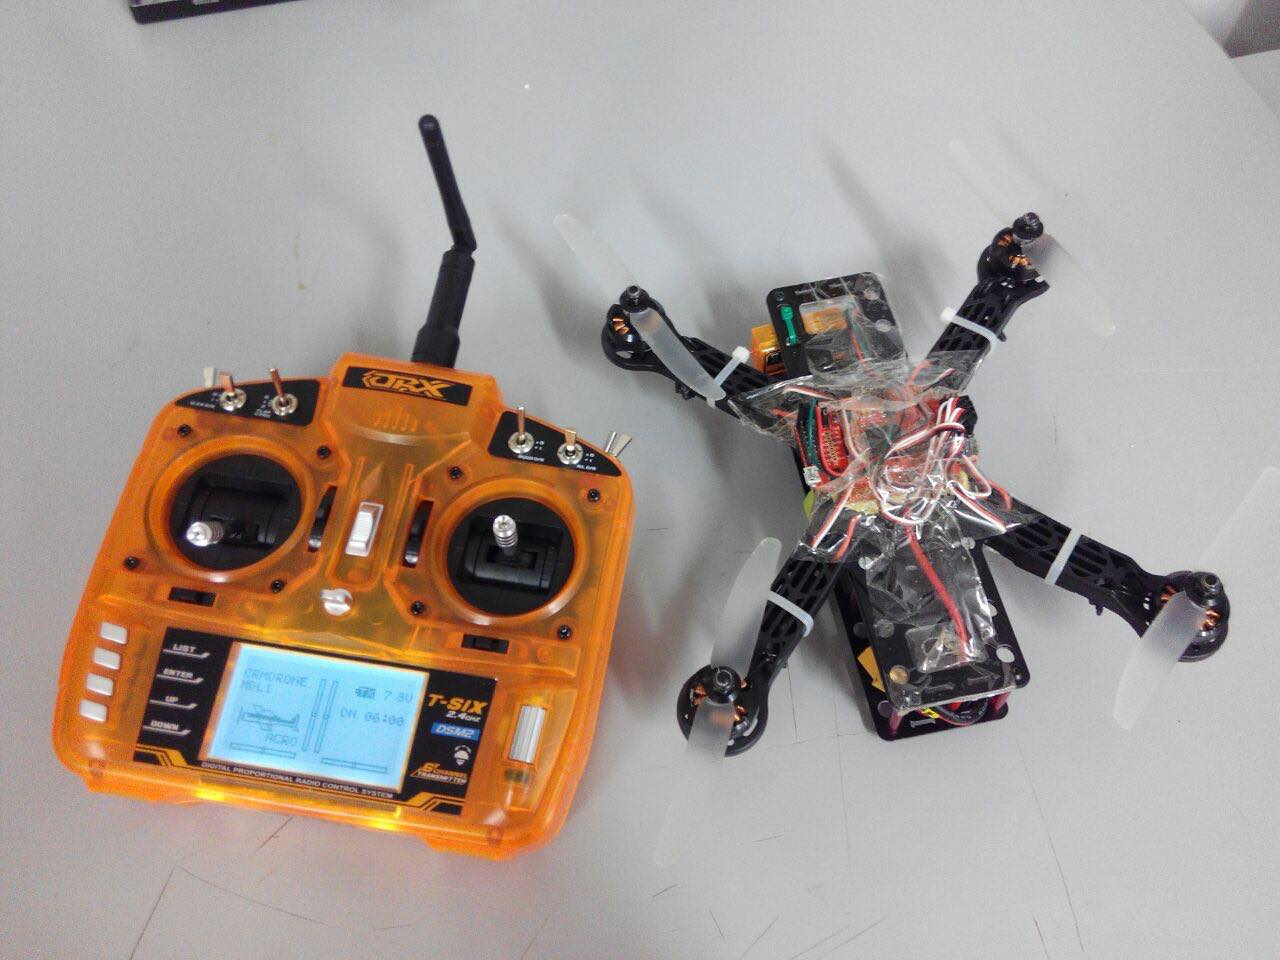
\includegraphics[scale=0.16]{fotos/dron1.jpg}
    \caption*{}
\end{wrapfigure}
Durante el curso 2014-15 realizamos desde el Club de Robótica el proceso de diseño, compra de materiales, y montaje de un cuadricóptero.
Éste tipo de robots son capaces de volar gracias a cuatro hélices actuadas por motores de alta velocidad.

Aunque es posible comprar éstos dispositivos ya montados, hemos preferido construir nuestra propia versión para así poder aprender más a fondo cómo funciona ésta tecnología.

En los meses de febrero y abril realizamos las compras de los materiales presupuestados, y durante el proceso nos encontramos con agunas dificultades en los trámites aduaneros, lo que alargó el proceso en tiempo y dinero. A pesar de los problemas, ésto fue algo positivo ya que nos ayudó a aprender la forma correcta de tramitar los pedidos de material electrónico al extranjero.

Una vez tuvimos todos los materiales a punto, nos reunimos para realizar el montaje de la estructura mecánica del robot usando una configuración estándar para cuadricópteros (configuración en H).

Con el cuadricoptero ya montado, llegó el turno de soldar las conexiones de la electrónica. La placa controladora principal está basada en el firmware abierto \emph{multiWii}, que tuvimos que programar y configurar para el vuelo.
En las primeras pruebas detectamos un problema con uno de los motores, ya que se calentaba demasiado al girar, pero nos dimos cuenta de que los problemas los estaban causando unos tornillos demasiado apretados.

Una de las tareas más costosas en tiempo y delicadas fue, a partir de la construcción completa, el ajuste preciso de los parametros de vuelo para conseguir un buen balance entre estabilidad y agilidad.

\begin{figure}[hbtp]
\centerline{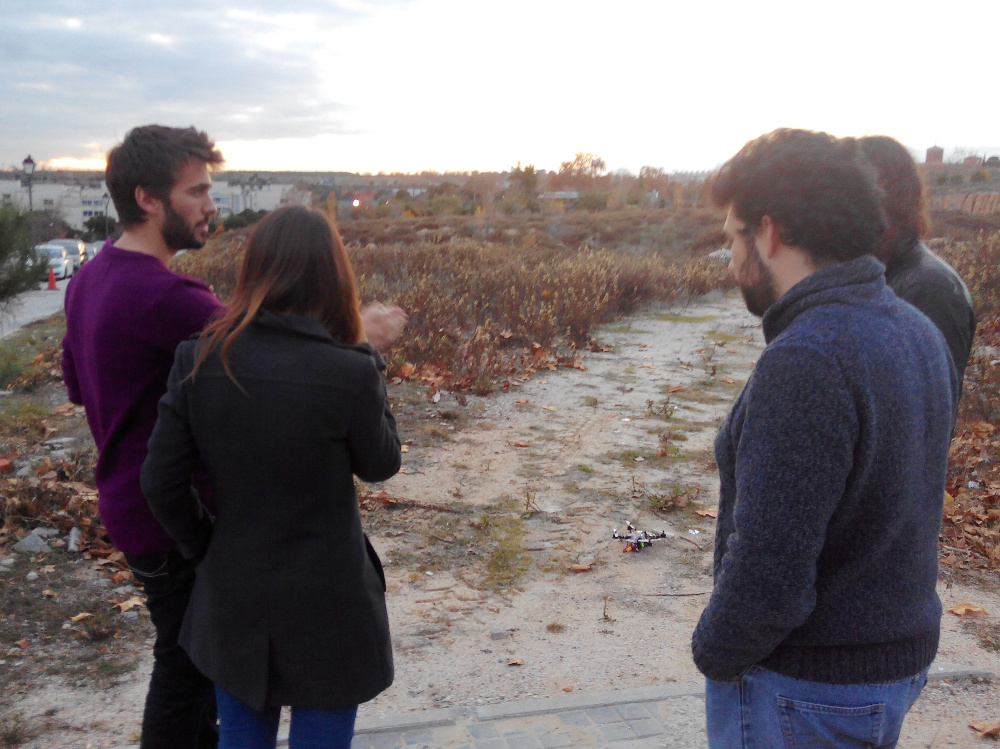
\includegraphics[width=0.6\linewidth]{fotos/2015-12-11_PruebaVuelo_JaimeCrisPabloRafa.jpg} 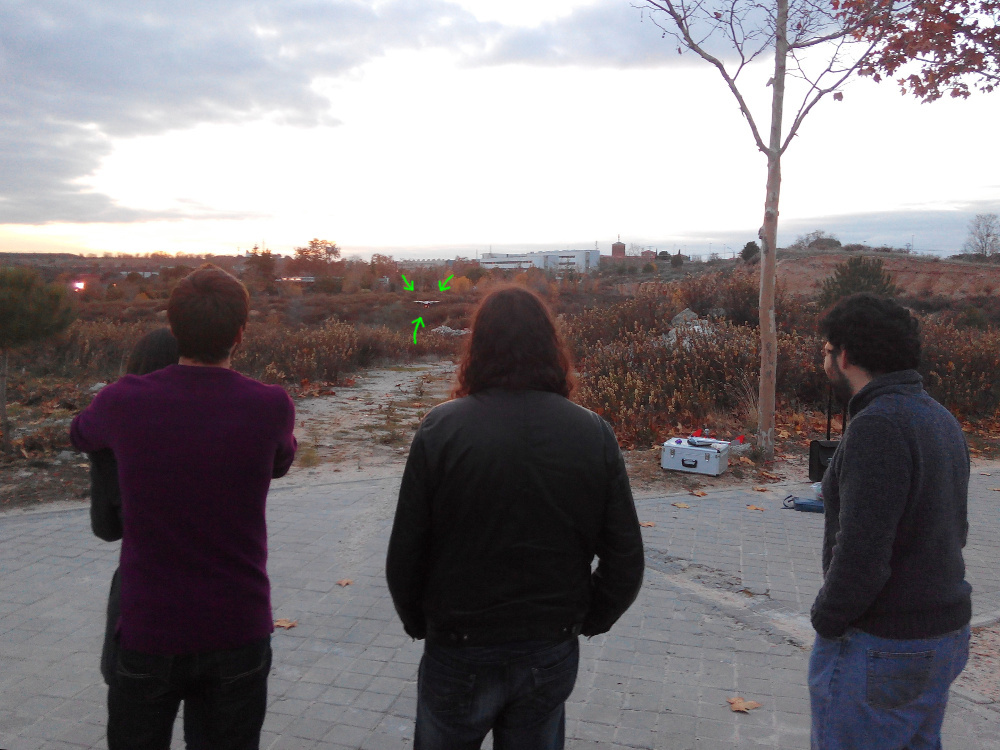
\includegraphics[width=0.6\linewidth]{fotos/2015-12-11_PruebaVuelo_CrisJaimeRafaPablo.jpg}}
\caption*{
Pruebas de vuelo de nuestro cuadrucóptero en una explanada del campus situada detrás del edificio C de la Escuela Politécnica Superior. Por supuesto tomamos todas las medidas de seguridad necesarias durante las pruebas.
}
\end{figure}

No sólo aprendimos a construir un robot capaz de volar, ¡también fue necesario aprender a calibrarlo y pilotarlo!
Para ello contamos con la gran experiencia del jefe de proyecto Jaime Aragón, un gran entusiasta de los drones de radio-control. Jaime nos dio varias clases de vuelo e incluso hizo demostraciones de vuelo de alta velocidad con sus drones dotados de FPV (First Person View, es decir, con cámara en primera persona).

El siguiente paso de éste proyecto va a ser la automatización del control del cuadrucóptero (hacerlo autónomo en lugar de tele-operado) mediante la incorporación de sensores; ésto lo hemos detallado en la sección de presupuestos para el nuevo curso.





\subsection{Uso de nuestra impresora 3D por estudiantes de la comunidad universitaria}

Desde el Club de Robótica intentamos fomentar el uso de la impresora 3D que construimos en 2014 para todos los miembros de la comunidad universitaria.

Además de la valiosa labor que realiza la impresora para el Club (ya que, tanto los robots diseñados para los talleres, como los proyectos ya detallados, usan estructuras impresas 3D) durante este año la impresora ha servido a múltiples alumnos y personal investigador para realizar prototipos de proyectos tecnológicos.

\begin{figure}[hbtp]
\centerline{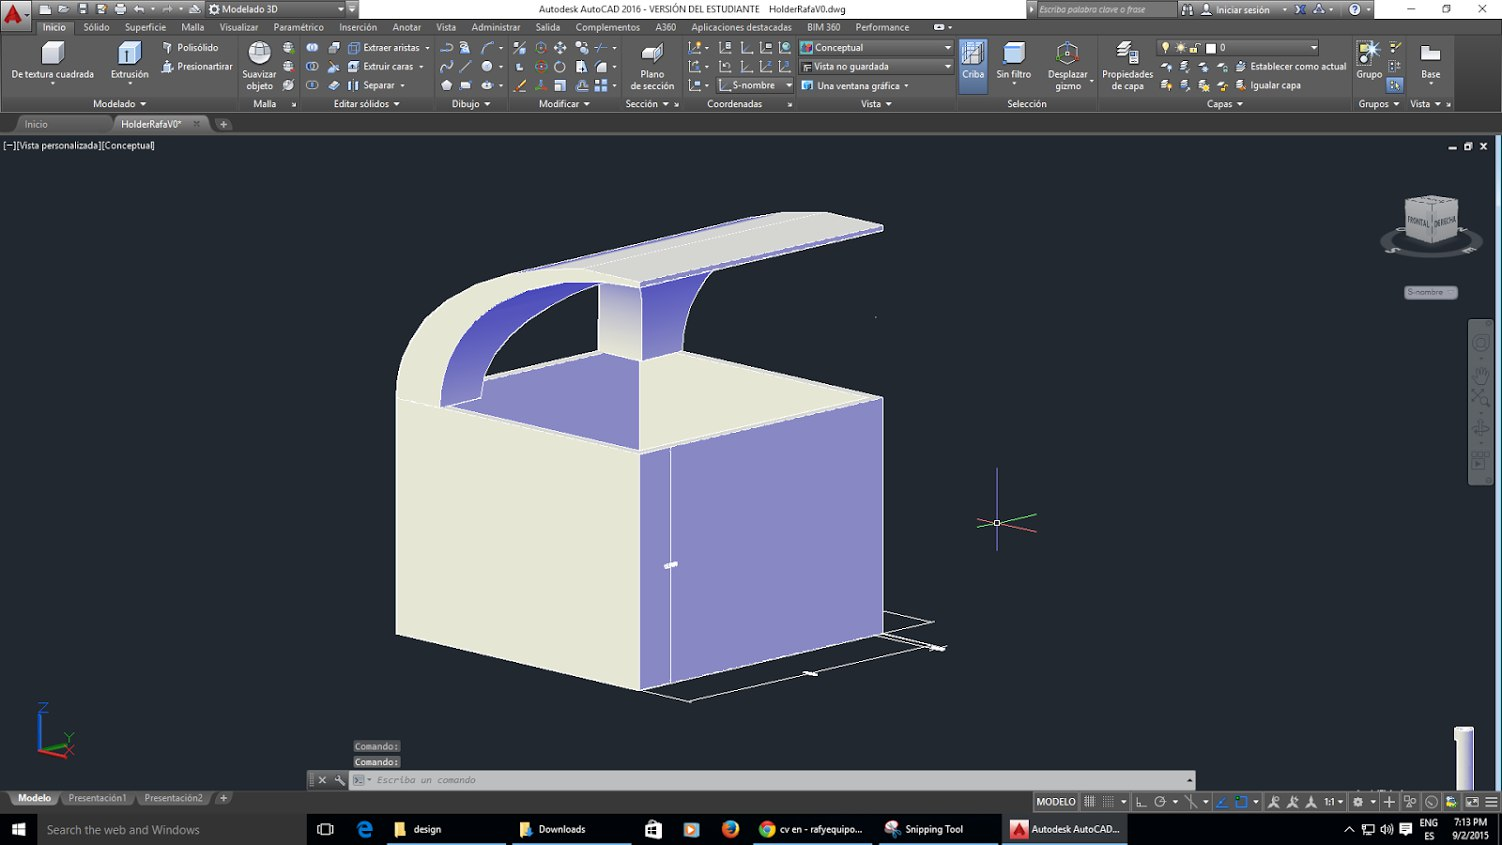
\includegraphics[width=0.4\linewidth]{fotos/impresora1.jpg} 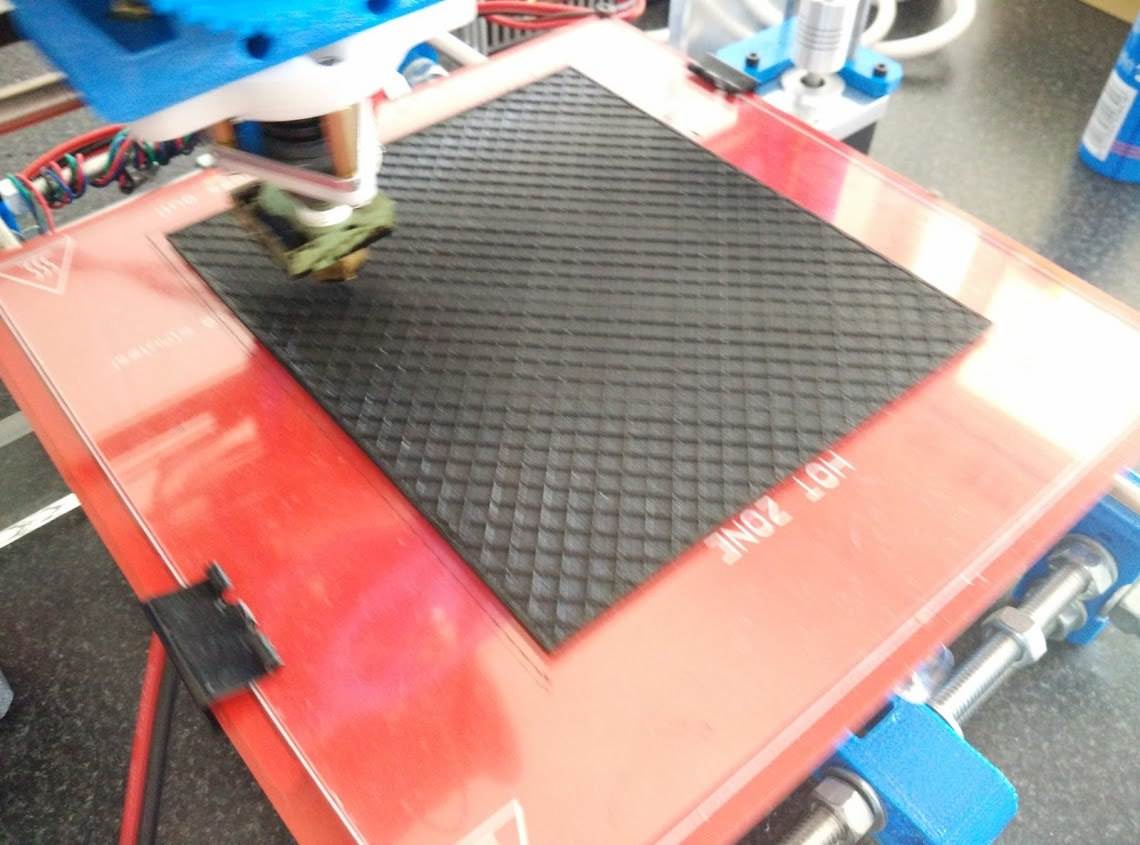
\includegraphics[width=0.35\linewidth]{fotos/impresora2.jpg} 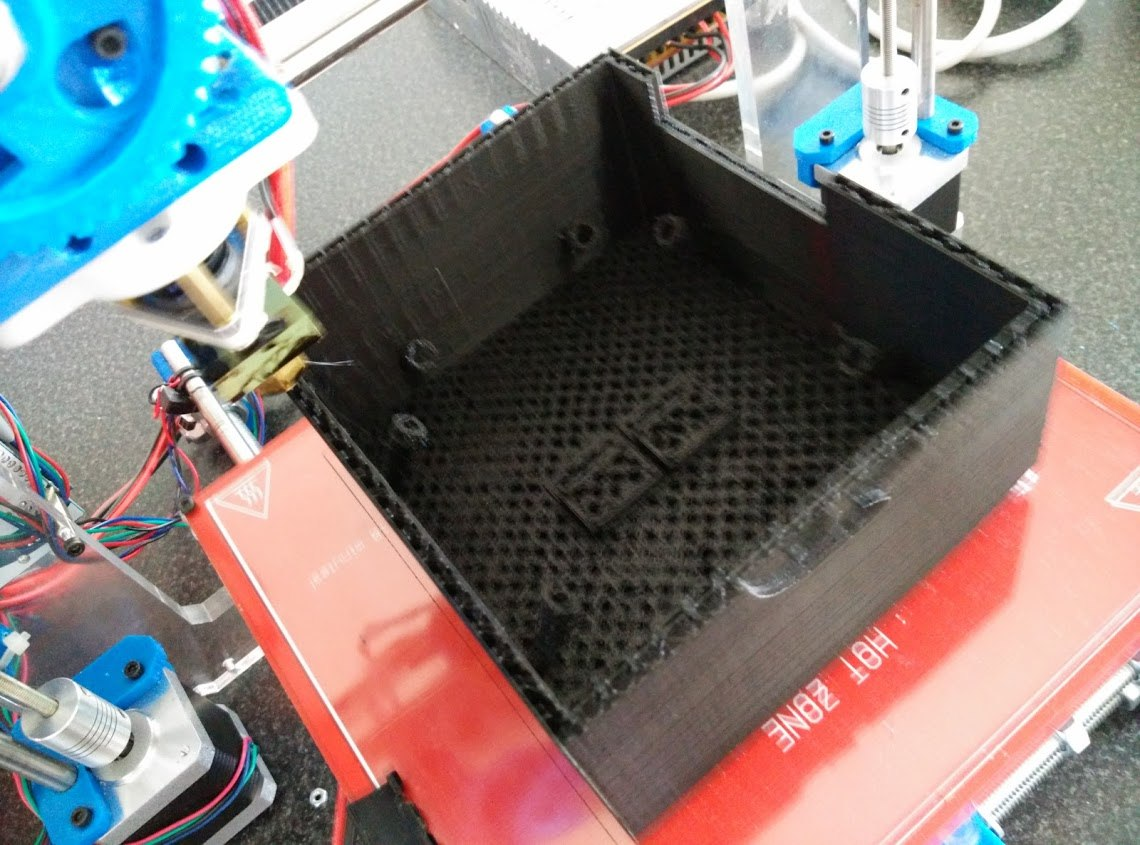
\includegraphics[width=0.4\linewidth]{fotos/impresora3.jpg}}
\centerline{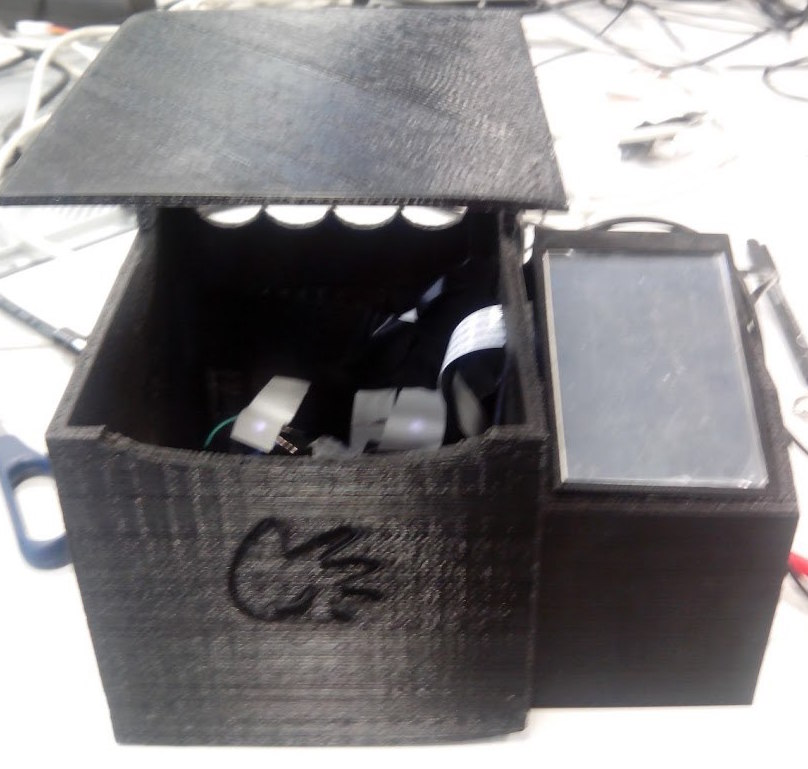
\includegraphics[width=0.4\linewidth]{fotos/impresora4.jpg}}
\caption*{
Proceso completo de diseño e impresión 3D de un \emph{escáner biométrico} para un proyecto de investigación colaborativo con una \emph{start-up} de la Escuela Politécnica Superior.
}
\end{figure}

Creemos que el disponer de herramientas como ésta otorga una gran libertad a los estudiantes para lanzarse a realizar proyectos propios que pueden llegar a alcanzar un gran éxito. Estamos intentando que la impresora 3D sea accesible a cualquier miembro de la comunidad universitaria, como ya sucede en otros centros (UPM, UC3M, UPC, Imperial College London, etc). Es por ello que para el próximo curso estamos organizando talleres interfacultativos de introducción al diseño e impresión 3D para las personas que tengan interés en aprender sobre éstas tecnologías.






%\subsection{Construcción de un robot para resolver laberintos}





\subsection{Re-organización del club para fomentar la participación}

Desde la junta directiva del Club de Robótica nos hemos propuesto dar nueva vida a la asociación, mejorando las condiciones de trabajo en nuestro local y documentando todas las actividades en una nueva página web.

\begin{figure}[hbtp]
\centerline{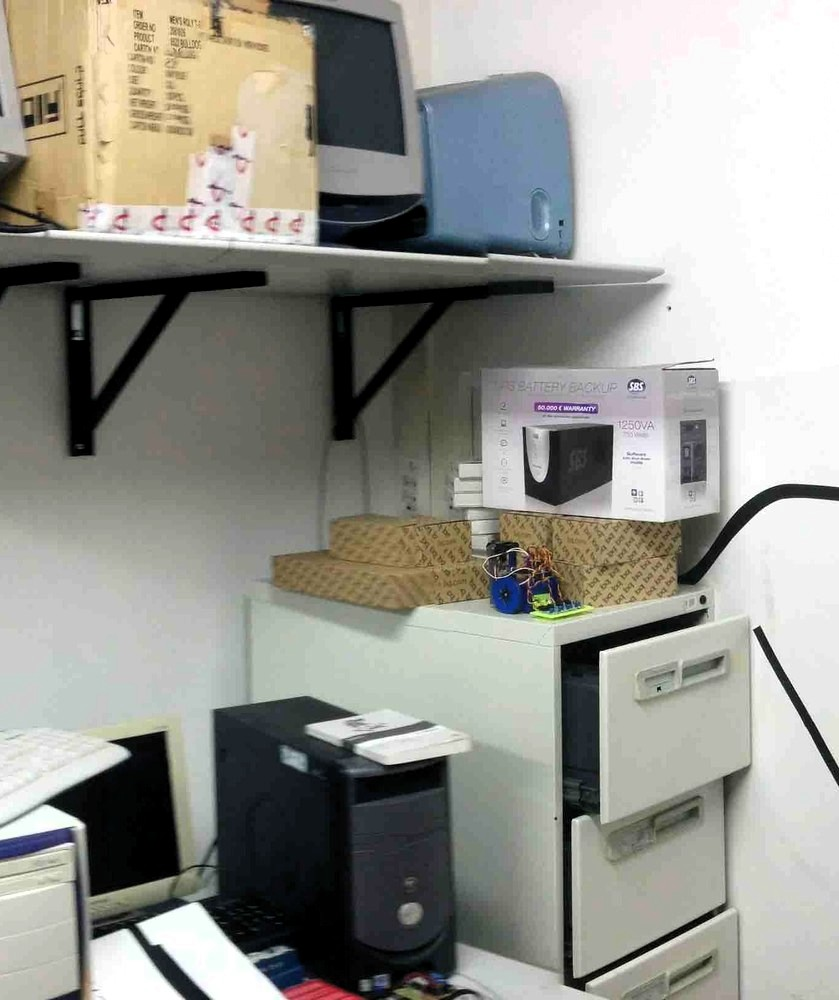
\includegraphics[width=0.36\linewidth]{fotos/tallerAntes3}
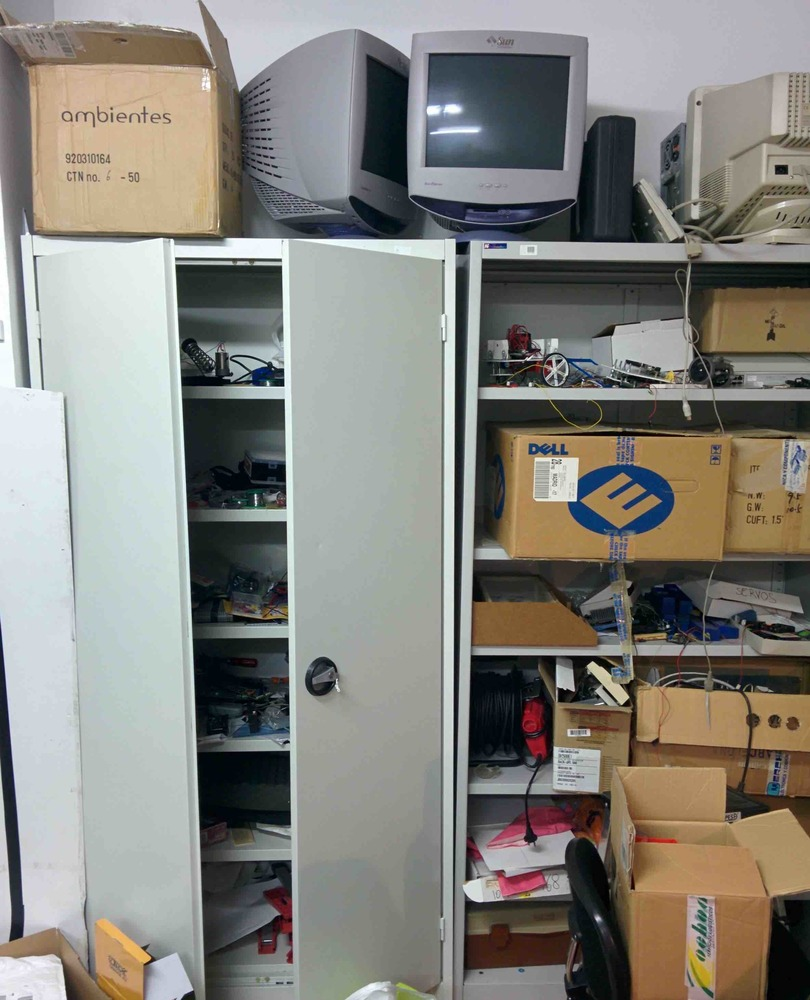
\includegraphics[width=0.35\linewidth]{fotos/tallerAntes1}
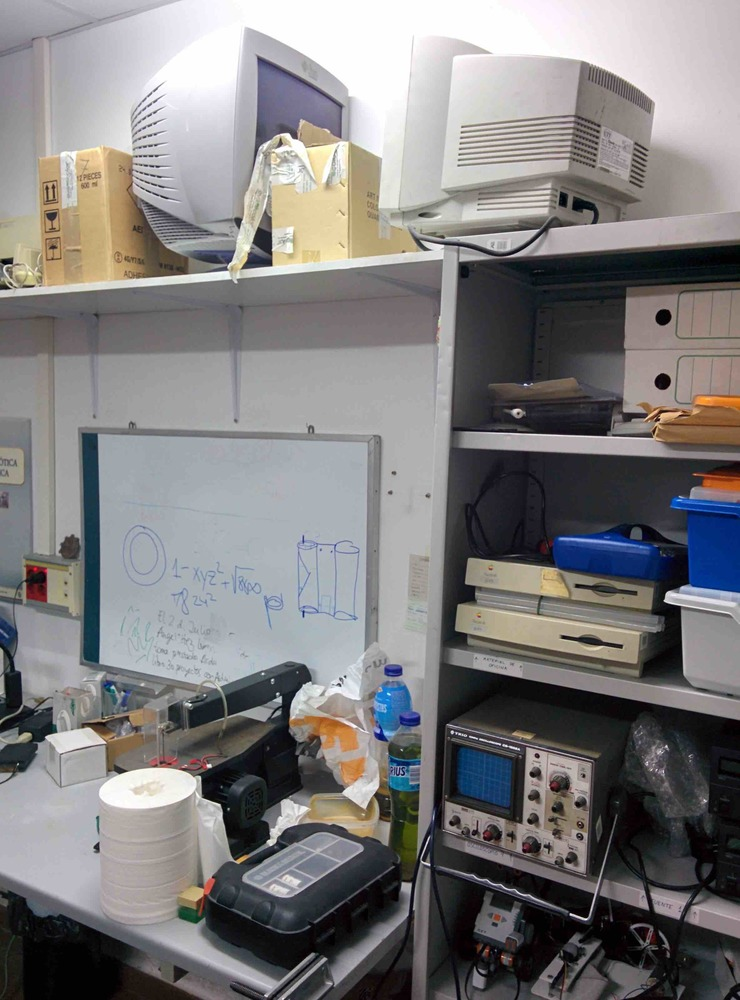
\includegraphics[width=0.32\linewidth]{fotos/tallerAntes2}}
\caption*{
El local de la asociación estaba en un estado bastante desastroso antes de la renovación, lo que limitaba la actividad debido a la falta de orden y espacio
}
\end{figure}

\begin{figure}[hbtp]
\centerline{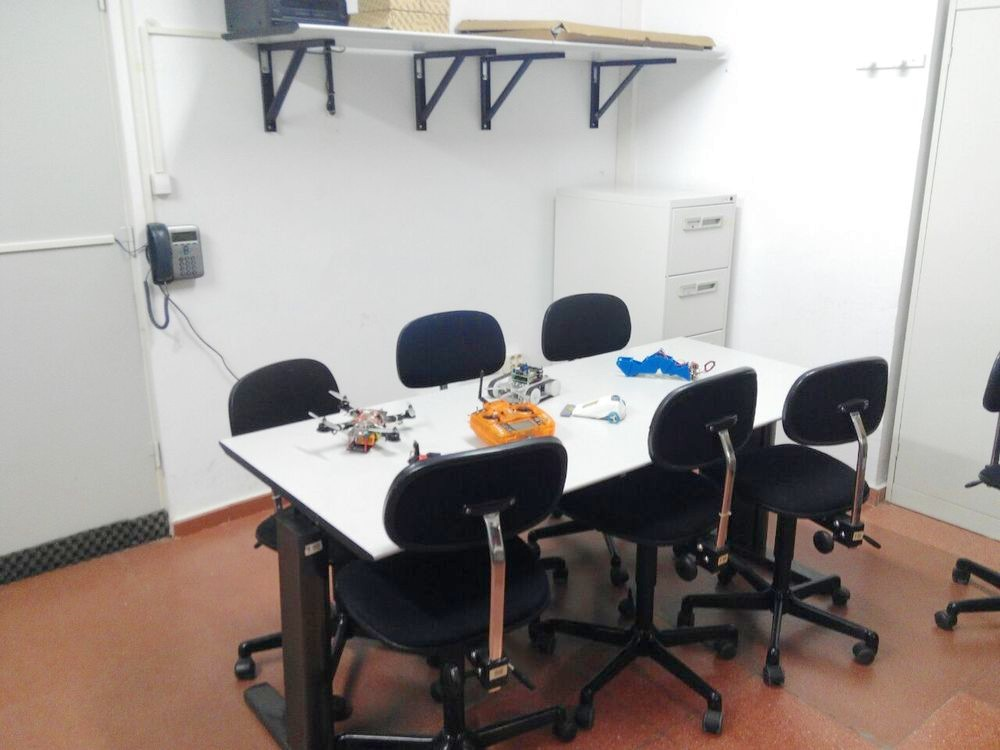
\includegraphics[width=0.45\linewidth]{fotos/tallerDespues5}
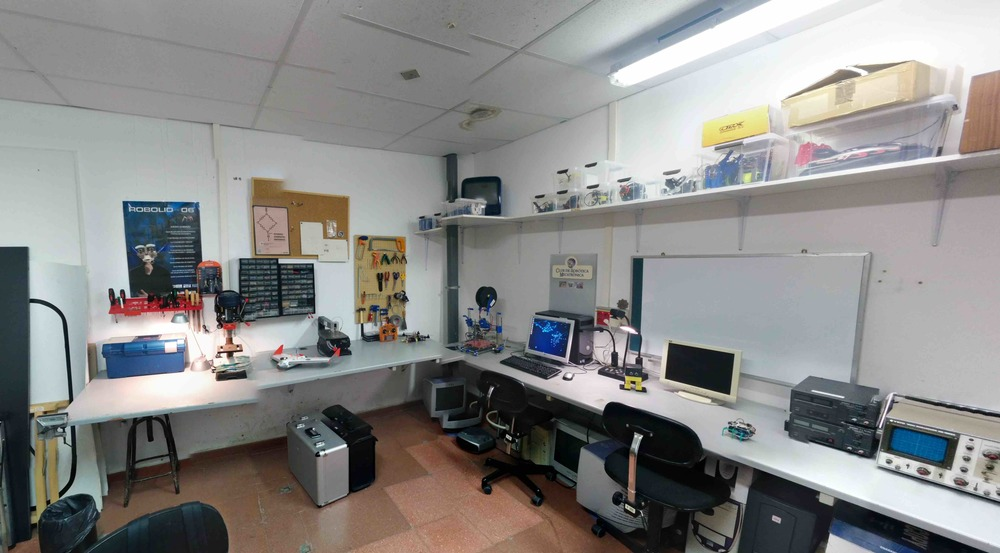
\includegraphics[width=0.75\linewidth]{fotos/tallerDespues3}}
\caption*{
Tras la renovación, el local por fin es un sitio amplio y agradable donde pueden trabajar varias personas simultáneamente.
}
\end{figure}


Para renovar el Club de Robótica hemos realizado las siguientes tareas:

\begin{itemize}
\item Actualización de la página web y creación de repositorio GitHub para el control de versiones. \textbf{La nueva web puede verse en \url{http://crm.ii.uam.es}}, y nuestro repositorio colaborativo es \url{http://github.com/CRM-UAM}
\item Limpieza del local (reciclado de equipos obsoletos que ocupaban espacio, mesas despejadas para facilitar la labor del equipo de limpieza)
\item Organización del material de los armarios y de las herramientas gracias a un panel de madera con ganchos y cajas de plástico modulares (éste material lo compramos con parte del presupuesto disponible)
\end{itemize}

El nuevo enfoque del Club de Robótica es apoyar a cualquier miembro de la comunidad universitaria que quiera llevar a cabo proyectos relacionados con la robótica. Es decir, tanto estudiantes como profesores pueden inscribirse y así disponer de un espacio de trabajo agradable con herramientas de uso común (impresoras 3D, soldadores, sierras, alicates, destornilladores, etc) así como los materiales necesarios (cables, componentes, motores, baterías, etc).

Para ello la idea es que cada miembro puede solicitar una caja de proyecto donde guardar todo el material que necesite. Dichas cajas se etiquetan con el año, nombre de proyecto, y del responsable; de este modo es posible organizar mejor el inventario disponible.

%\begin{figure}[hbtp]
%\centerline{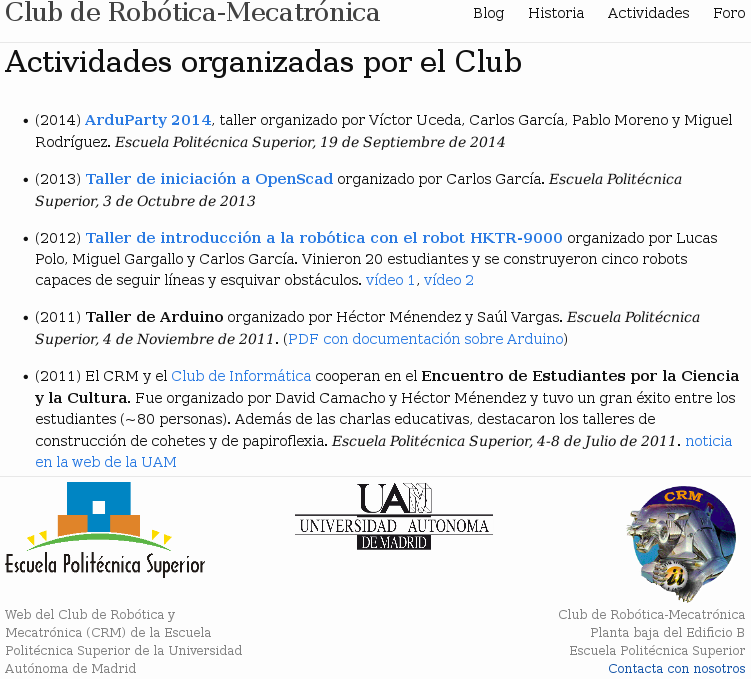
\includegraphics[width=0.75\linewidth]{fotos/web}}
%\caption*{
%Nueva web institucional del Club de Robótica, integrada en un repositorio %GitHub de desarrollo colaborativo
%}
%\end{figure}

\begin{wrapfigure}[10]{l}{8cm}\centering
    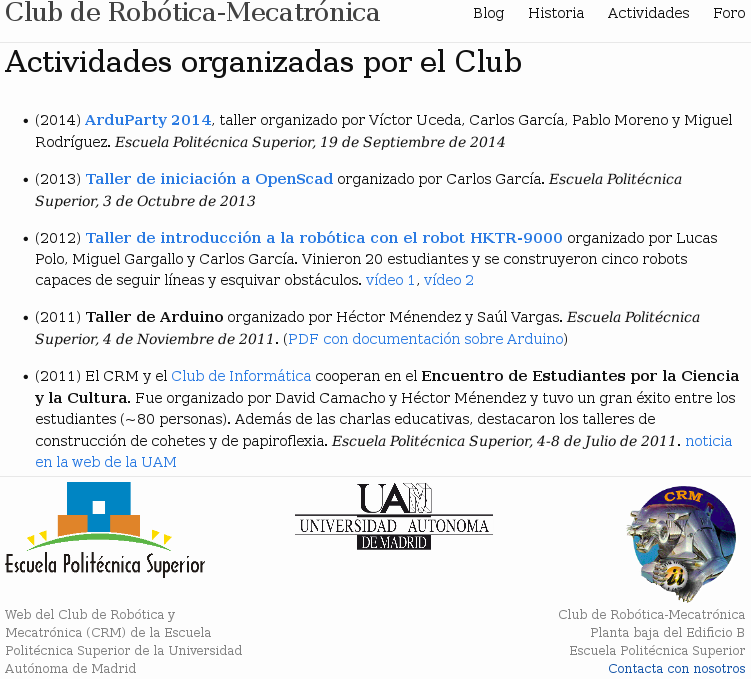
\includegraphics[scale=0.3]{fotos/web}
    \caption*{}
\end{wrapfigure}

Además hemos creado un foro/lista de correo para gestionar la asociación, así como ayudarnos unos a otros con nuestros proyectos.

Gracias al nuevo foro, la web renovada y a la re-organización del local, esperamos que aumente la participación en el club y así se realicen más actividades de fomento de la robótica en la Universidad Autonóma.




\newpage

\section{Participación en eventos nacionales}


\subsection{Concurso de resolución de laberintos en la OSHWDem (Galicia, A Coruña)}

La OSHWDem (Open Source Hardware Demonstration) es un evento que se realiza anualmente en A Coruña. Allí se reúnen estudiantes e investigadores de diversas disciplinas, y entre otras cosas se organizan competiciones de robótica\footnote{\url{http://oshwdem.org/concursos/}}.

\vspace{5mm}

\centerline{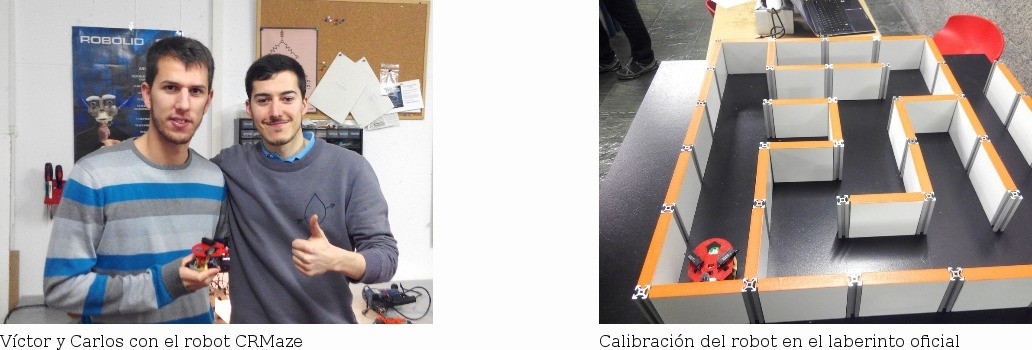
\includegraphics[width=1.1\linewidth]{fotos/oshwdem2015_robot}}

Éste año nos propusimos presentar un robot al concurso de resolución de laberintos (también conocido como \emph{micromouse}). Fue todo un reto porque tan sólo tuvimos dos semanas para construir el robot y programar los algoritmos necesarios.
El resultado fue el robot CRMaze\footnote{\url{https://github.com/CRM-UAM/CRMaze}}.


\vspace{5mm}
\centerline{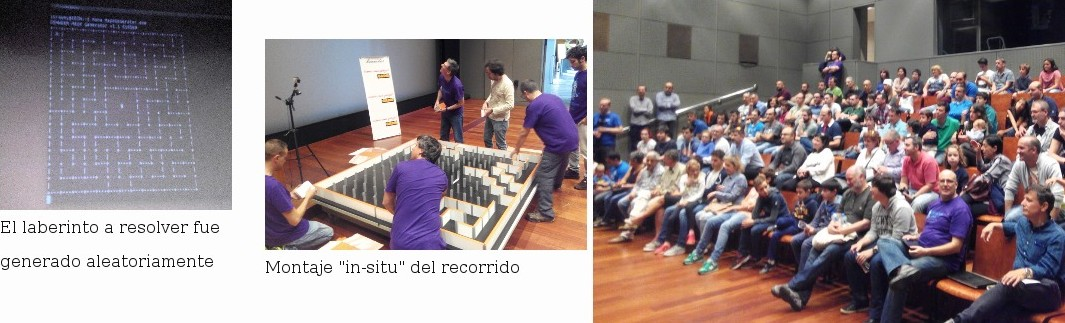
\includegraphics[width=1.1\linewidth]{fotos/oshwdem2015_laberinto}}


Aunque ninguno de los participantes fue capaz de resolver el laberinto debido a su alta complejidad, fue una experiencia muy interesante y todos aprendimos mucho. Además recibimos un trofeo impreso en 3D con filamentos de cobre y bronce.


\begin{wrapfigure}[10]{l}{7cm}\centering
    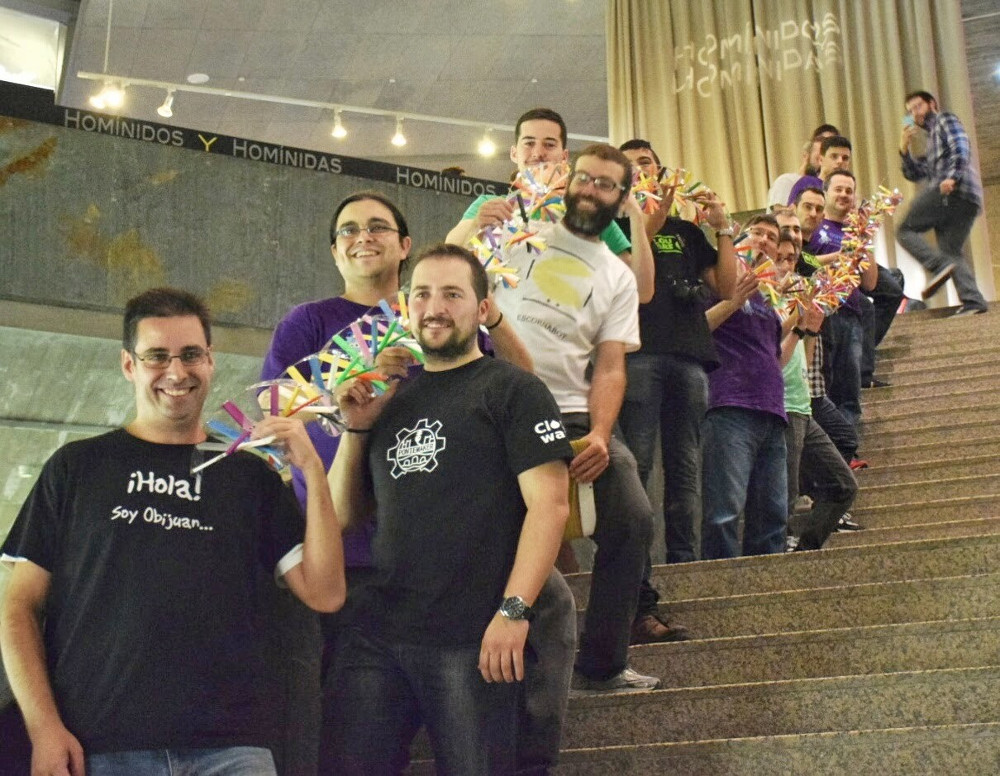
\includegraphics[scale=0.2]{fotos/2015_OSHWDem_cadenaADNcloneWars}
    \caption*{}
\end{wrapfigure}
También participamos en el reto \emph{ADN CloneWars}\footnote{\url{https://github.com/brico-labs/RetoADNCloneWars}}. En él se imprimieron más de 500 piezas para construir una cadena de ADN con los nombres de todas las impresoras open-source construidas en España dentro del grupo RepRap Clone Wars\footnote{\url{www.reprap.org/wiki/Clone_wars}}.

El Club de Robótica forma una parte importante de la cadena ya que el clon Nº5, \emph{Halcón Milenario}, fue construido en 2012 en el local de la asociación.

Para el curso que viene nos hemos propuesto mejorar el diseño del robot CRMaze para conseguir resolver el laberinto por fin, y además queremos crear más equipos que participen en el resto de concursos dentro de la OSHWDem (categorías de seguidores de línea, robots de sumo y de combate, además de la de resolución de laberintos).



\subsection{Asistencia a la V jornada GMV de robótica (Madrid, Tres Cantos)}


El 26 de Noviembre de 2015 asistimos desde el Club de Robótica al evento que tuvo lugar en la sede oficial de GMV, situada en Tres Cantos. Allí se realizaron demostraciones en directo de los robots Foxiris (para monitorización de plantas oil \& gas), MiR100 (un robot de exploración de tipo rover) y Aunav (un robot usado para la desactivación de explosivos)\footnote{\tiny\url{http://www.gmv.com/es/Empresa/Comunicacion/NotasDePrensa/2015/NP_017_VJornadaRobotica.html}}.

\begin{figure}[hbtp]
\centerline{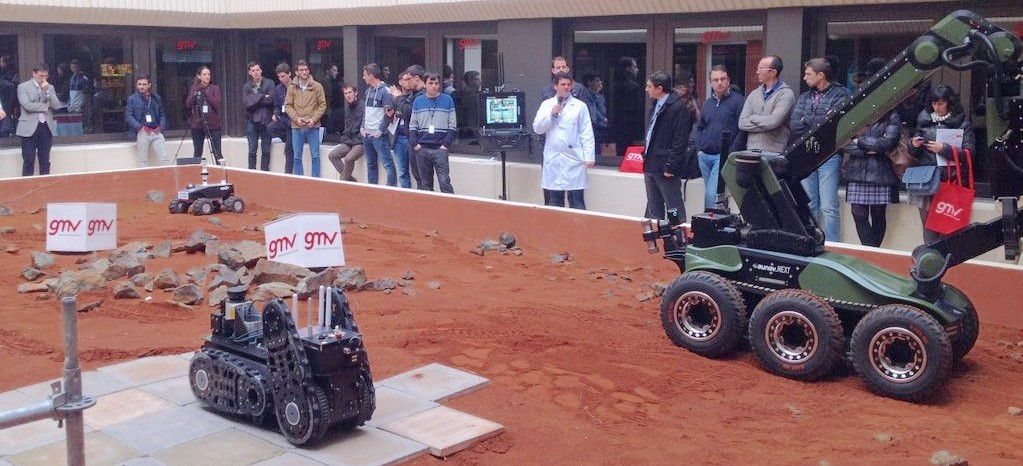
\includegraphics[width=0.75\linewidth]{fotos/2015_V_JornadaRobotica_GMV}}
\caption*{
Demostración de los robots Foxiris de GMV (izquierda), MiR100 de Robotplus (al fondo) y Aunav de Proytecsa (derecha).
}
\end{figure}

Además volvimos a representar a la Autonóma, ésta vez en el concurso ``Concurrent Design Facility (CDF) for Robotics'' en el que se nos asignó la tarea de diseñar un robot para la monitorización de plantas oil \& gas en menos de tres horas. Obtuvimos el primer premio junto con estudiantes de la UPM.


\begin{figure}[hbtp]
\centerline{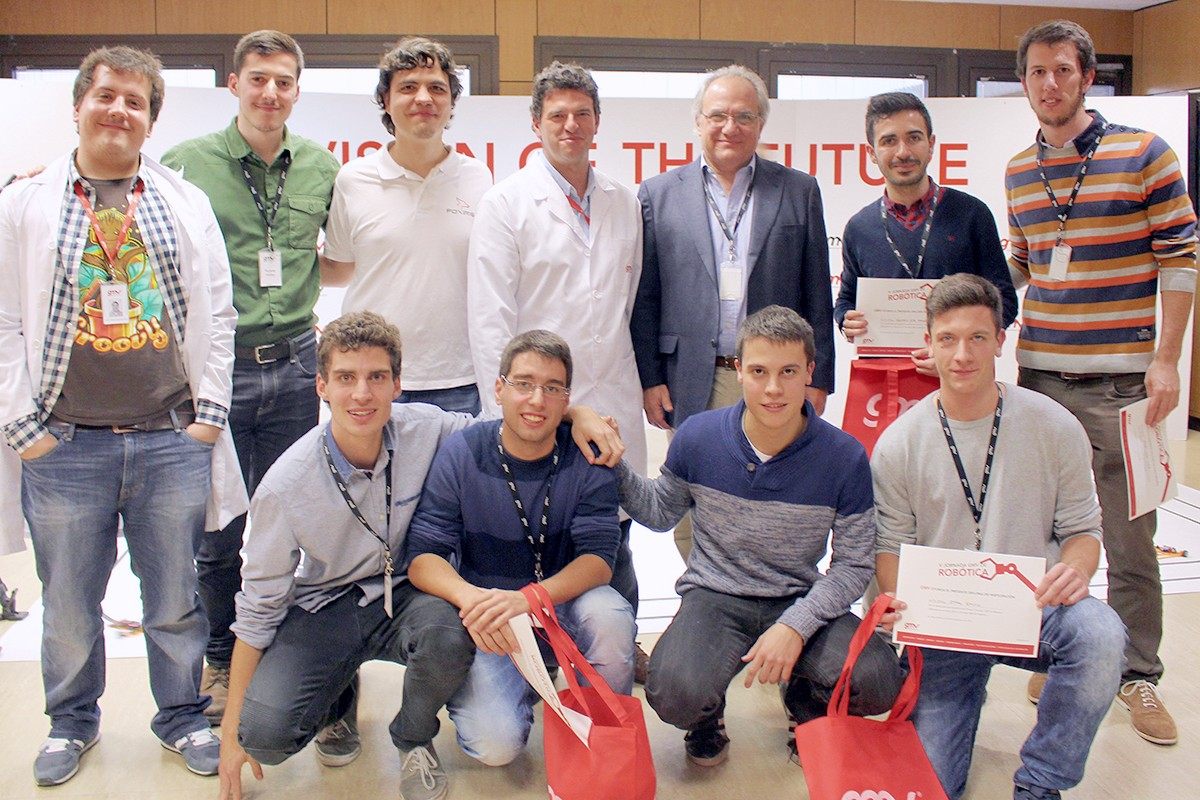
\includegraphics[width=0.75\linewidth]{fotos/2015_V_JornadaRobotica_GMV_team}}
\caption*{
Participantes en el concurso ``Concurrent Design Facility (CDF) for Robotics''. \\
Fila superior: Carlos Crespo (GMV), Carlos García (CRM-UAM), Sergio Martini (GMV), Alberto Medina (GMV), Pedro Hernández (Repsol), Gonzalo Díaz (UPM) y Víctor Uceda (CRM-UAM)
Fila inferior: Luis Paarup, David Matilla, Javier Fernández, Stefan y Pablo Rodríguez -ausente en la foto- (todos de la UPM)
}
\end{figure}


El curso que viene seguiremos buscando activamente éste tipo de eventos para garantizar que la Universidad Autonóma tenga representación estudiantil en el ámbito de la robótica a nivel nacional.




%%%%%%%%

\chapter{Presupuesto para nuevas actividades}


Para el curso 2015-2016 hemos empezado con energías renovadas gracias al éxito del año anterior con el proyecto del cuadricóptero. Nos hemos propuesto terminar de renovar el local de la asociación para mejorar las condiciones -y así fomentar la participación de los estudiantes-, organizar talleres formativos, y por supuesto seguir construyendo robots capaces de participar en diversas competiciones a nivel nacional.


\section{Actividades y talleres para el curso 2015-16}

\subsection{Material y herramientas para el local}

Consideramos muy necesario realizar una compra del siguiente material, de cara a finalizar la renovación de la asociación, proporcionar un ambiente limpio y ordenado, y garantizar que hay espacio suficiente para que los nuevos miembros almacenen sus proyectos sin interferirse unos a otros:

\begin{itemize}
\item \textbf{Cajas organizadoras transparentes grandes (21x30x40cm)}, que cuestan 4.25\euro{}/u. Estimamos necesarias 5 cajas, lo que hace un total de 21.25\euro{}.
\item \textbf{Cajas de proyecto pequeñas (14x19x29cm)}, que cuestan 2.95\euro{}/u. Estimamos necesarias 20 cajas, lo que hace un total de 59\euro{}.
\item \textbf{Aspirador de polvo portátil} para facilitar la limpieza de las mesas y estanterías. El modelo que nos interesa cuesta 39.90\euro{}.
\item \textbf{Sistema extractor de aire} para la ventilación del local ya que no tiene ventanas, es particularmente necesario para filtrar los humos producidos al soldar con estaño. Las piezas necesarias para construirlo (filtros, tubos, ventiladores) cuestan en torno a 30\euro{}.
\item \textbf{Herramientas de medida precisas y alicates de corte}, ya que los que tenemos están defectuosos. Un set de tres calibres electrónicos y cuatro alicates de corte sale por 70\euro{}, y se podrán utilizar en los talleres de impresión 3D.
\end{itemize}

Por tanto, para dicha renovación estimamos necesarios \textbf{220.15\euro{}}.



\subsection{Adaptación del cuadricóptero para vuelo autónomo}
\subsubsection{Responsable de proyecto y equipo de trabajo}
\begin{itemize}
\item Rodrigo Jimenez, Estudiante de Telecomuniciones, EPS.
\item Cristina Kasner, estudiante de Informática-Matemáticas, EPS.
\item Carlos García, estudiante de doctorado, EPS.
\item Guillermo Ruíz, estudiante de Informática-Matemáticas, EPS.
\item Jaime Aragón, Estudiante de Telecomuniciones, EPS.
\item Víctor Uceda, estudiante de Informática-Matemáticas, EPS.
\end{itemize}
\subsubsection{Descripción y objetivos}
Tal y como se detalla en la memoria de actividades, el año pasado presentamos un presupuesto para la construcción de un drone.

Como recordatorio la idea principal era construir un cuadricóptero manejado por control remoto capaz de detectar y evitar obstáculos en un modo de control autónomo.

Durante el pasado año académico completamos con éxito la primera parte del proyecto y ya tenemos construido y calibrado el cuadricóptero que ha pasado satisfactoriamente las primeras pruebas de vuelo teleoperado.


\begin{figure}[hbtp]
\centerline{
    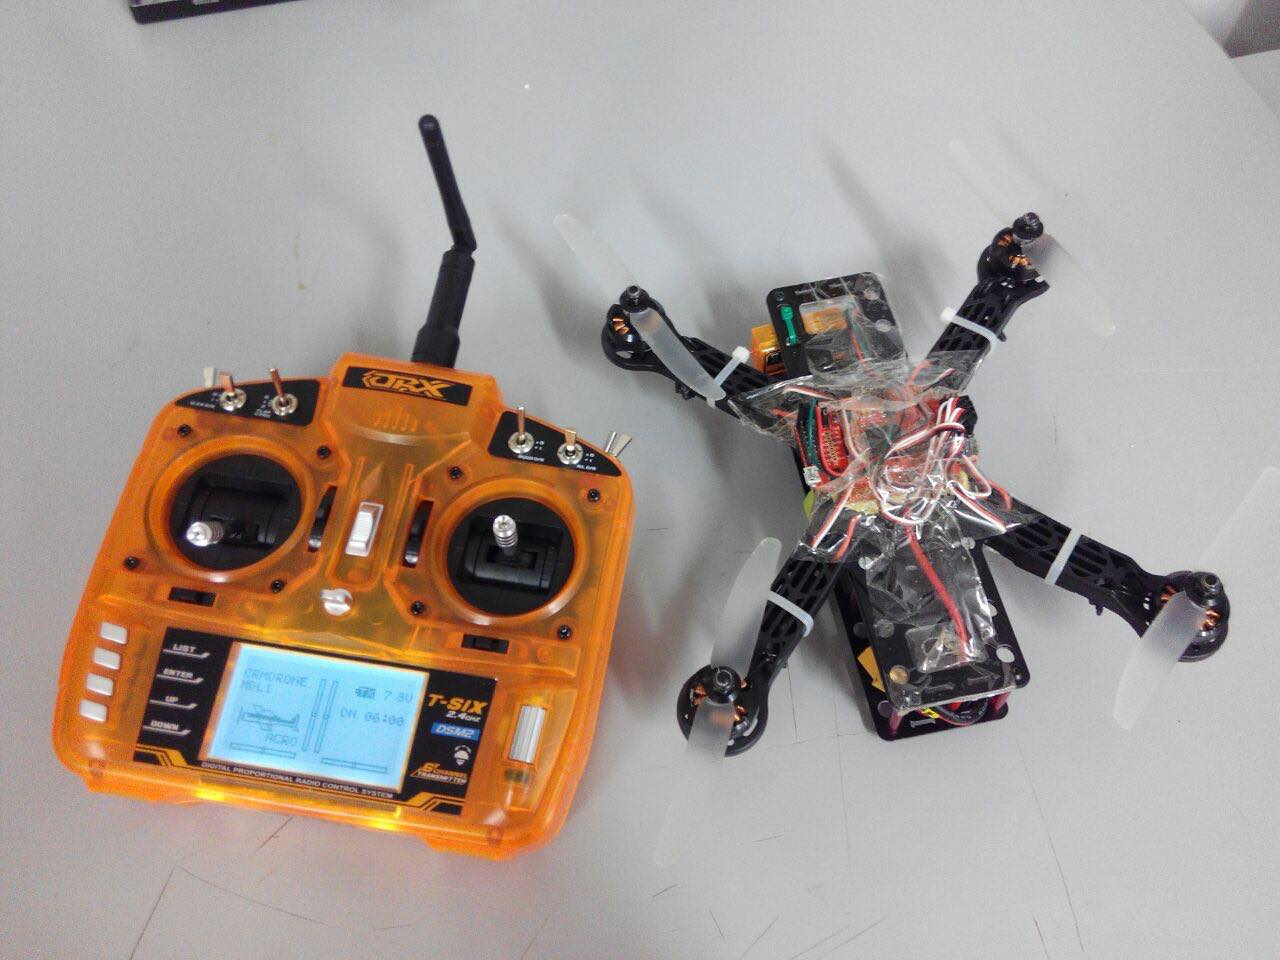
\includegraphics[width=0.45\linewidth]{fotos/dron1.jpg}
    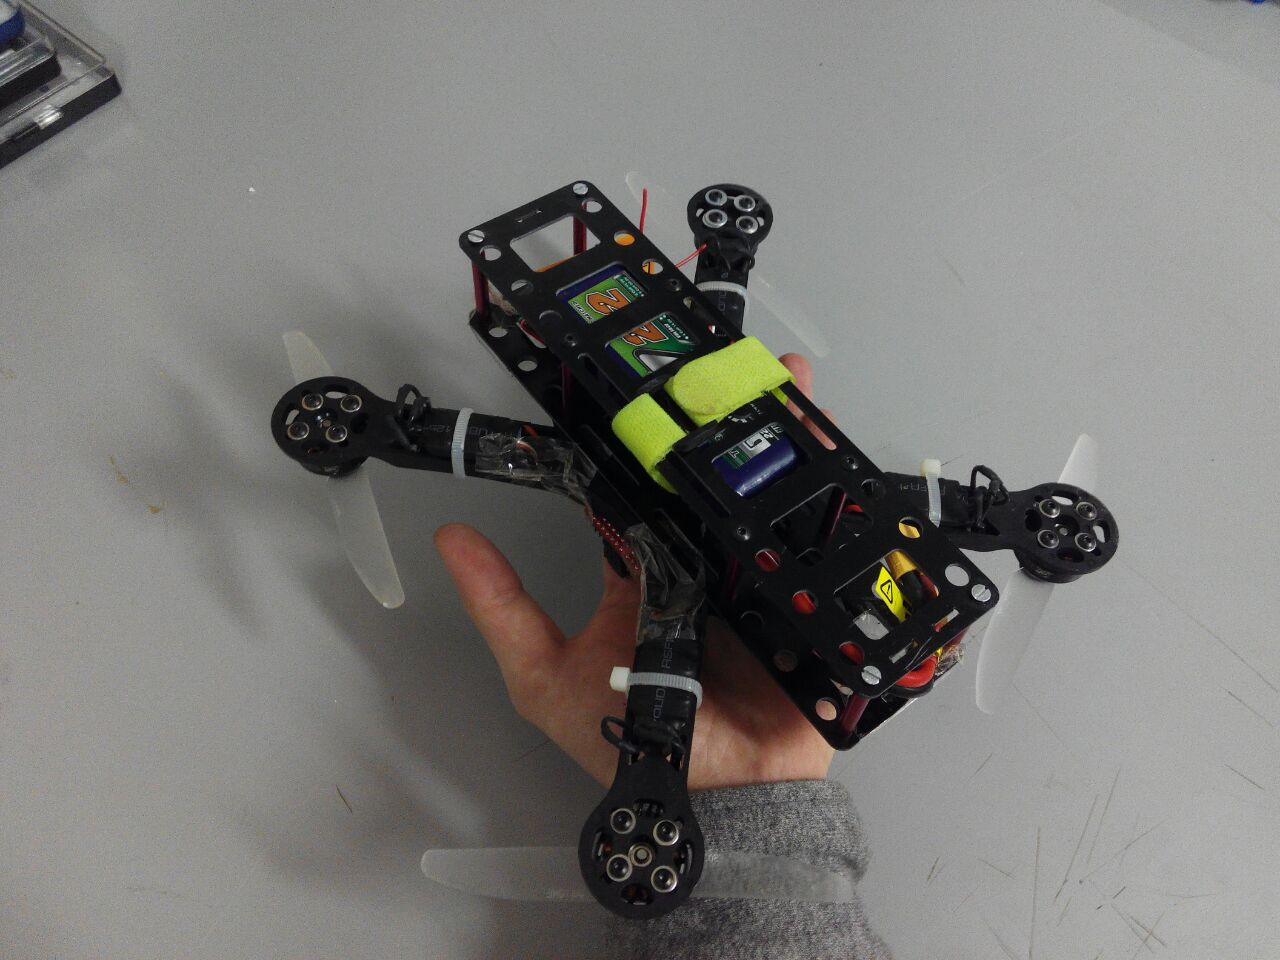
\includegraphics[width=0.45\linewidth]{fotos/dron2.jpg}}
\caption*{
Fotos del estado actual de nuestro cuadrucóptero}
\end{figure}

Queremos por tanto duante este próximo curso proseguir con el proyecto realizando el módulo de vuelo autónomo.


\subsubsection{Detalles y Contenido}
Nuestra intención es filtrar las señales que llegan al receptor del cuadricóptero mediante las medidas de los sensores ultrasónicos y con ayuda de la arduino para evitar posibles colisiones.

Existen numerosos cuadricópteros comerciales que disponen de GPS y son semi-autónomos (es decir, se les proporcionan unas coordenadas como objetivo y el robot realiza la ruta deseada), pero normalmente funcionan en campo abierto y sin obstáculos.

Por eso queremos marcar la diferencia e intentar diseñar uno de los primeros cuadricópteros que no solo fuesen capaces de ir hasta unas determinadas coordenadas en campo abierto, sino que fuese capaz de detectar los obstáculos que se encuentre a su paso y los evite, modificando la ruta inicial gracias a los sensores y los cálculos realizados en tiempo real por nuestros algoritmos.


\subsubsection{Previsión de desarrollo}
En la primera parte de este proyecto nos hemos dedicado exclusivamente a la fabricación de un Drone básico para lo cual hemos comprado las partes principales como son la estructura, motores, variadores, bateria, mando, receptor, y la controladora de vuelo (con GPS). Una vez concluida satisfactoriamente esta primera parte , es decir, habiendo construido el cuadricoptero y lograr pilotarlo, nos disponemos a pedir presupuesto para la continuación de este proyecto.

Al empezar este proyecto parecía algo ambicioso y difícil de llevar a cabo pero hemos construido un drone completamente funcional y lo hemos calibrado para que tenga unas condiciones de vuelo óptimas, por lo que vemos mucho más cerca el poder llevar a cabo la idea inicial y comenzar este año con el reto de que sea capaz de volar de manera autónoma e incluso disponer de unas gafas de realidad virtual FPV (\emph{First Person View}).

Ésta es nuestra meta debido a que sería lo que realmente diferenciaría nuestro trabajo de otros proyectos: La idea de que sea completamente autónomo es pionera en el campo y debido a la diversidad de estudiantes (Ingeniería de Telecomunicación, Informática y doble grado de Informática y Matemáticas) creemos que tenemos los conocimientos necesarios para llevarlo a cabo.

\subsubsection{Presupuesto}
El año pasado el coste de las piezas se disparó debido a unos gastos de aduanas imprevistos, por lo que únicamente pudimos construir el drone (sin elementos de visión artificial ni sensores necesarios para el vuelo autónomo) concluyendo así lo que podríamos denominar la primera parte del proyecto.

Enumeramos a continuación los elementos presupuestados para esta segunda fase, junto con su precio, enlace de compra y la descripción y justificación:

\begin{itemize}
\item  {\bf Sensor de distancia por ultrasonidos [x6] 18,03\euro{}/u}

Enlace: \url{www.electan.com/sensor-distancia-por-ultrasonidos-ping-p-3134.html}

Con estos sensores pretendemos detectar obstaculos en cualquiera de las seis direciones posibles de movimiento del dron (norte, sur, este, oeste, y los dos movimientos verticales) creando un mapa virtual de obtaculos y pudiendo así evitarlos modificando la ruta óptima lo menos posibles.

\centerline{
    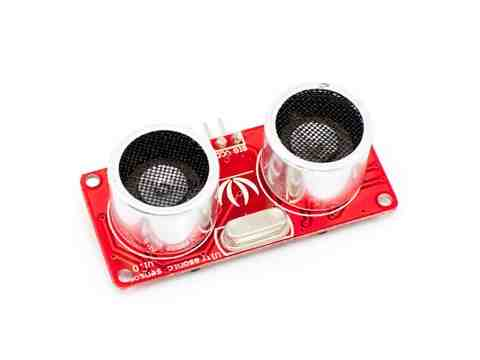
\includegraphics[width=0.45\linewidth]{fotos/sensor_ultra.jpg}}

\item {\bf Hélices eficientes (HQ 6") [x3 packs] 5,30\euro{}.}

Enlace: \url{flyduino.net/Multikopter-Propeller-CW-CCW_44}

Sin duda las hélices  son las partes del drone que más expuestas a colisiones están. Por ello pedimos presupuesto para comprar 3 juegos de este tipo hélices, que además son de una calidad alta lo que disminuirá el riesgo a que se partan, pero aun así, es seguro, que necesitaremos recambios.

\centerline{
    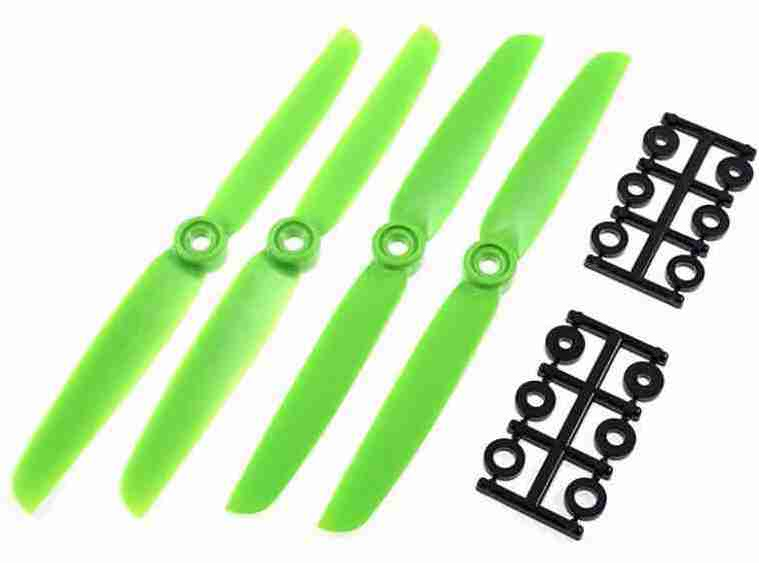
\includegraphics[width=0.45\linewidth]{fotos/helices.jpg}}

\item {\bf Cámara y transmisor de imagen. [x2] 29\euro{}/u.}

Enlace: \url{www.rctimer.com/product-1318.html}

Esta será la cámara y el transmisor de video que nos permitirá grabar la imagen y transmitirla a tiempo real a las gafas de realidad virtual.

\centerline{
    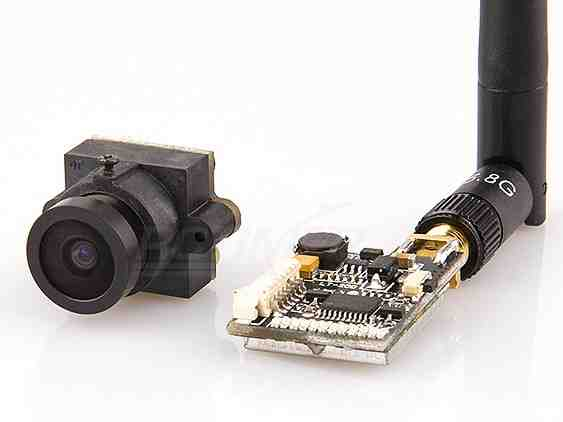
\includegraphics[width=0.45\linewidth]{fotos/camara.jpg}}


\item {\bf Módulo receptor de imagen. 28\euro{}.}

Enlace: \url{www.hobbyking.com/hobbyking/store/__83195__Fat_Shark_Raceband_5_8GHz_Module.html}

Con este módulo podemos recibir la imagen enviada por el dron para procesarla en el ordenador o mandar a las gafas de realidad aumentada del operador.

\centerline{
    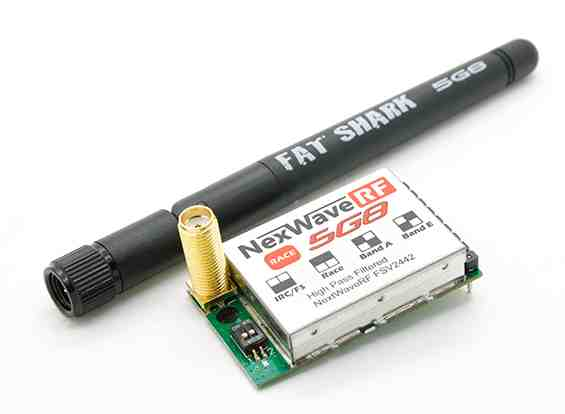
\includegraphics[width=0.45\linewidth]{fotos/receptor.jpg}}

\item {\bf Antenas de polarización circular. 20\euro{}.}

Enlace: \url{www.rctimer.com/product-1099-index.html}

Las antenas que incluyen el transmisor y el módulo receptor son de polarización lineal y nos podrían provocar problemas debido a los cambios de orientación del drone por lo que queremos comprar estas antenas de polarización circular que con un precio bastante asequible nos permitirían alcanzar más del doble de distancia sin distorsiones.


\centerline{
    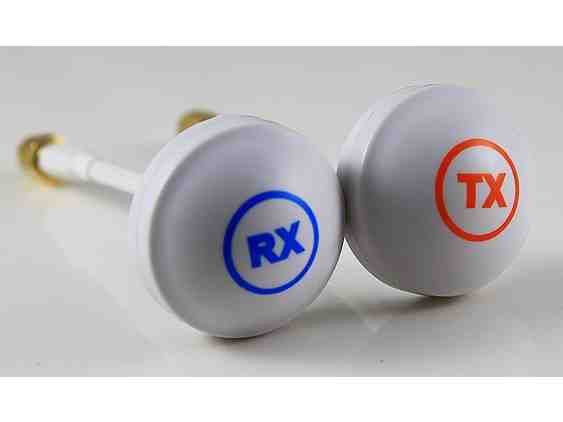
\includegraphics[width=0.45\linewidth]{fotos/antena.jpg}}

\item {\bf Gafas de realidad aumentada FPV. 320\euro{}.}

Enlace: \url{www.hobbyking.com/hobbyking/store/__84640__Fatshark_Dominator_V3_Headset_EU_Warehouse_.html}

Estas gafas son necesarias para poder pilotar el drone y monitorizar la telemetría en primera persona (First Person View). Sabemos que son un elemento caro, pero esto nos abrirá numerosas puertas para el futuro ya que como se observa en los anteriores componentes el transmisor y la cámara son bastante baratos y podríamos realizar numerosos proyectos donde dar utilidad a estas gafas de realidad virtual. Una de las muchas ventajas que tienen estas  gafas son por ejemplo unos acelerómetros que nos permitirán girar la cámara del drone (instalando dos servos) con el movimiento de nuestra cabeza, lo que daría una sensación de inmersión total.

\centerline{
    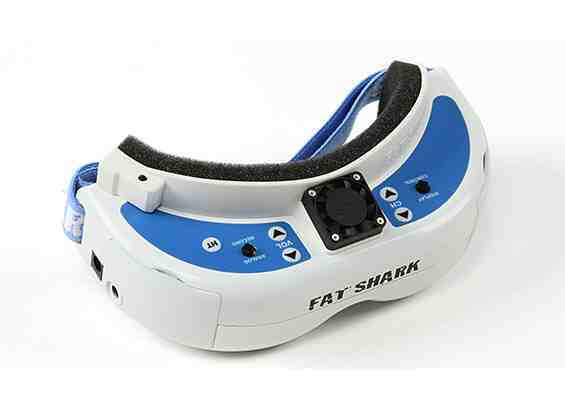
\includegraphics[width=0.45\linewidth]{fotos/gafas.jpg}}

\end{itemize}

En total, el presupesto estimado para completar el proyecto del cuadrucóptero (incluyendo gastos de envío previstos, aduanas, etc) se estima en \textbf{579\euro{}}.








\subsection{Construcción Fresadora Cyclone PCB}
\subsubsection{Equipo de trabajo}
\begin{itemize}
\item Carlos Garcia, estudiante de doctorado, EPS.
\item Rodrigo Jimenez, estudiante de Telecomuniciones, EPS.
\item Pablo Molins, personal investigador, EPS.
\item Víctor Uceda, estudiante de Informática-Matemáticas, EPS.
\end{itemize}
\subsubsection{Descripción}
Aspiramos a conseguir un Club de Robótica completamente funcional que permita a los socios realizar proyectos de robótica de una forma rápida y eficiente, para ello creemos fundamental agilizar el tránsito desde la idea incial de un proyecto a los primeros protipos funcionales.

Para ello queremos contar con las tres herramientas modernas fundamentales: impresora 3D (ya disponible en el taller), fresadora (capaz de realizar circuitos electrónicos impresos) y un escáner 3D.

\subsubsection{Objetivos}
Desarrollar esta herramienta que promete ser tan útil para el CRM, a la par de perfeccionar nuestros conocimientos de electrónica y montaje ya que tendremos que unicamente adquirir las piezas en un kit (basado en un proyecto de Open Hardware).

\subsubsection{Motivación}
Por el momento, como no disponemos de ésta herramienta, tenemos que realizar nuestros circuitos de una forma muy artesanal (y muy poco eficiente), el proceso que seguimos actualmente es el siguiente:
\begin{enumerate}
\item Diseñar el circuito eléctrico en el ordenador (esta fase se mantiene)
\item Imprimir en papel fotográfico el circuito
\item Planchar el circuito sobre la placa de cobre para lograr la transferencia de la tinta y que el circuito quede ``impreso'' en tinta sobre la placa
\item Sumergir la placa en ácidos para que se elimine el cobre que la recubre (salvo en las zonas protegidas por la tinta) quedando el circuito en cobre finalmente conectado
\item Taladrar manualmente todos los agujeros de la placa
\item Finalmente, cortar el PCB a la medida necesaria
\end{enumerate}

Con la fresadora Cyclone éstos pasos se simplifican ya que se trata de una máquina CNC que trabaja de forma autónoma y además no necesita emplear componentes químicos nocivos.



\subsubsection{Previsión de desarrollo}

\begin{wrapfigure}[11]{r}{6.5cm}\centering
    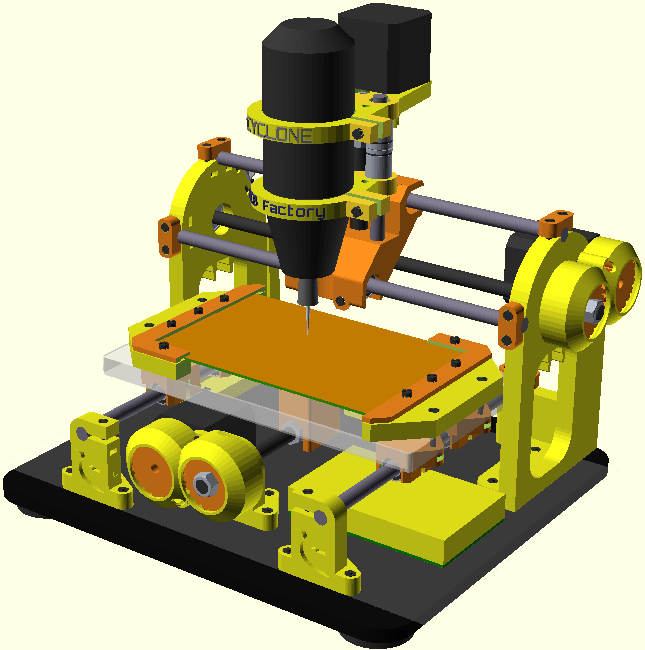
\includegraphics[scale=0.32]{fotos/Cyclone}
    \caption*{}
\end{wrapfigure}

Vamos a montar el kit distribuido por bq, basado en el proyecto open-source Cyclone PCB que se encuentra ampliamente documentado en: \url{https://github.com/carlosgs/Cyclone-PCB-Factory}

Una vez adquirido el kit y cuando lo tengamos disponible en nuestro taller, nos reuniremos para realizar el montaje y calibración.
Después pasaremos a la fase de testeo de la máquina, documentando en la web las instrucciones de uso con tutoriales de fabricación de PCBs.

\subsubsection{Presupuesto}
El kit es ditribuido por bq (\url{store.bq.com/es/cyclone}) con un coste total de {\bf 499\euro{}} y gastos de envío gratuitos.









\newpage

\subsection{Construcción de un Escáner 3D modelo Ciclop}

\subsubsection{Equipo de trabajo}
\begin{itemize}
\item Rodrigo Jiménez, estudiante de Telecomuniciones, EPS.
\item Pablo Moreno, estudiante de Informática-Matemáticas, EPS.
\item Víctor Uceda, estudiante de Informática-Matemáticas, EPS.
\end{itemize}
\subsubsection{Descripción}
 Tal y como hemos descrito en el proyecto anterior (fresadora Cyclone) necesitamos herramientas modernas y automáticas que agilicen un tránsito veloz desde las ideas a los prototipos funcionales.

Con este objetivo construimos la primera impresora 3D de la universidad. Creemos que la impresora 3D, junto a un escáner 3D y la fresadora Cyclone (que permite fresar circuitos electrónicos) son las herramientas modernas fundamentales para este proceso ágil.

\subsubsection{Objetivos}


\begin{wrapfigure}[11]{r}{6.5cm}\centering
    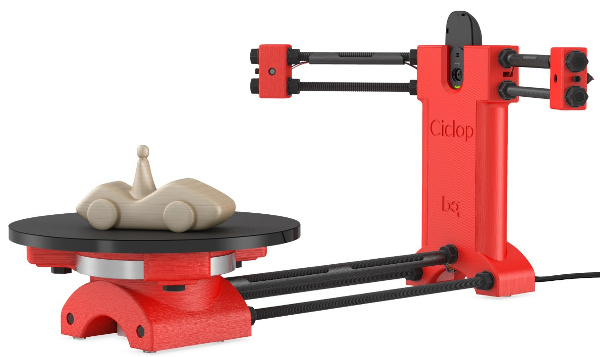
\includegraphics[scale=0.4]{fotos/bq-ciclop-1}
    \caption*{}
\end{wrapfigure}

Construcción del escáner 3D Ciclop diseñado y distribuido como kit de piezas por la empresa española BQ.\\
Además de adquirir una nueva herramiento de grandisima utilidad para el club, al ser un proyecto de construcción (ya que se compra el kit de piezas unicamente) tenemos el objetivo de aprender y profundizar en el diseño 3D, en la construcción de sistemas hardware y el software de escaneo y modelado 3D.
%\subsubsection{Contenido}

\subsubsection{Previsión de desarrollo}
La previsión de desarrollo del proyecto de montaje se estima en 2 semanas a partir del momento en el que el kit llegue al taller.\\
Con el escáner Ciclop ya montado comenzará la etapa de adaptación del software existente a los que equipos disponibles en el taller y la fase más importante de pruebas, calibrado y puesta a punto.
\subsubsection{Presupuesto}
La empresa BQ proporciona un kit completo de piezas los que nos permite acortar la étapa de adquisición de los materiales de forma muy notable e incluso ahorrar costes al adquirirlo todo en un mismo distribuidor.
El precio del kit es {\bf 249,90\euro{}}.
Enlace: \url{www.bq.com/es/ciclop}









\section{Organización de talleres formativos para alumnos de la Universidad}

Para el nuevo curso vemos viable la realización de los siguientes talleres:


\subsection{Taller: Introducción a las FPGAs libres con Verilog}
Las FPGAs son dispositivos empleados en aplicaciones que requieren velocidades de procesamiento muy elevadas debido a su alta potencia y reconfigurabilidad.
Recientemente se han desarrollado herramientas libres para trabajar con FPGAs, y desde el club de robótica queremos fomentar su uso ofreciendo uno de los primeros talleres del mundo en utilizarlas.

Queremos organizar el taller utilizando las placas \emph{iceStick} de Lattice Semiconductor:

\begin{figure}[hbtp]
\centerline{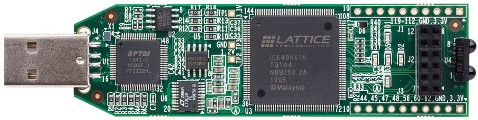
\includegraphics[width=0.75\linewidth]{fotos/icestick}}
\caption*{
Placa de desarrollo \emph{iceStick}
}
\end{figure}


Éstas placas tienen un coste muy reducido aún disponiendo de una FPGA de gran calidad. Además disponen de puerto USB para alimentación y datos, lo que las hace muy adecuadas para nuestro taller introductorio.

Para impartir el taller nos basaremos en los tutoriales que está realizando Juan González\footnote{\url{https://github.com/Obijuan/open-fpga-verilog-tutorial/wiki}}, antiguo profesor de la EPS-UAM. Éstos proporcionan una introducción muy didáctica y fácil de entender.

\subsubsection{Contenido}

\begin{itemize}
	\item Introducción teórica a las FPGAs, con ejemplos de uso práctico y demostraciones
	\item Explicación de las diferencias entre los lenguajes VHDL y Verilog
	\item Propuesta de ejercicios introductorios para resolver en parejas (generadores de frecuencias audibles y con diodos LED, sistemas DAC con PWM, etc)
	\item Explicación de algunos ejemplos más avanzados (generación de señales de puerto serie, control de un conversor analógico-digital, etc).
	\item Propuesta del reto: control de un robot usando la FPGA. Los estudiantes aprenderán a integrar las entradas y las salidas usando descripciones de hardware en Verilog.
\end{itemize}

Impartir éstos contenidos complementaría muy bien las asignaturas de FPGAs que se ofrecen actualmente en los grados de Telecomuniciones e Informática, ya que los lenguajes de programación Verilog y VHDL son ampliamente empleados en la industria.


\subsubsection{Presupuesto}

Cada placa \emph{iceStick} cuesta 21.28\euro{}, y para el taller necesitaríamos 10 unidades. Por ello, el presupuesto estimado es \textbf{212.8\euro{}} (los gastos de envío son gratuitos a partir de 50\euro{}).






\subsection{Taller: Diseño e Impresión 3D (Open Hardware)}
\subsubsection{Responsable de proyecto y equipo de trabajo}

\begin{itemize}
\item Cristina Kasner, estudiante de Informática-Matemáticas, EPS.
\item Víctor Uceda, estudiante de Informática-Matemáticas, EPS.
\item Carlos García, estudiante de doctorado, EPS.
\end{itemize}

\subsubsection{Descripción}
Se trata de un taller de modelado 3D orientado a la robótica, en el que se dará una introducción a los participantes del uso de la herramienta libre OpenSCAD para el diseño de piezas 3D. Además queremos realizar pequeños retos prácticos en los que los participantes puedan poner en práctica lo aprendido.

También se dará una charla sobre impresión 3D y finalizaremos mostrando como utilizar la impresora 3D existente en el club imprimiendo los mejores trabajos realizados por los participantes.
\subsubsection{Objetivos}
Queremos fomentar el diseño de open hardware entre los estudiantes de la universidad.

También queremos que los estudiantes aprendan utilizar la impresora 3D y sean libres de imprimir durante el curso piezas que necesiten para sus proyectos.

Por último queremos enseñar las ventajas y desventajas de imprimir con plástico o filamento de madera y cuándo puede ser útil cada uno de estos materiales


El contenido del curso será:
\begin{itemize}
	\item Introducción teórica a OpenSCAD
	\item Retos por parejas para poner en práctica lo aprendido.
	\item Exposición de los robots que se han construido con la impresora 3D en el CRM.
	\item Diseño libre por parejas de piezas imprimibles para la construcción de un robot.
	\item Explicación del funcionamiento y manejo de la impresora 3D.
	\item Impresión de los mejores diseños que hayan hecho los estudiantes.
\end{itemize}
\centerline{
	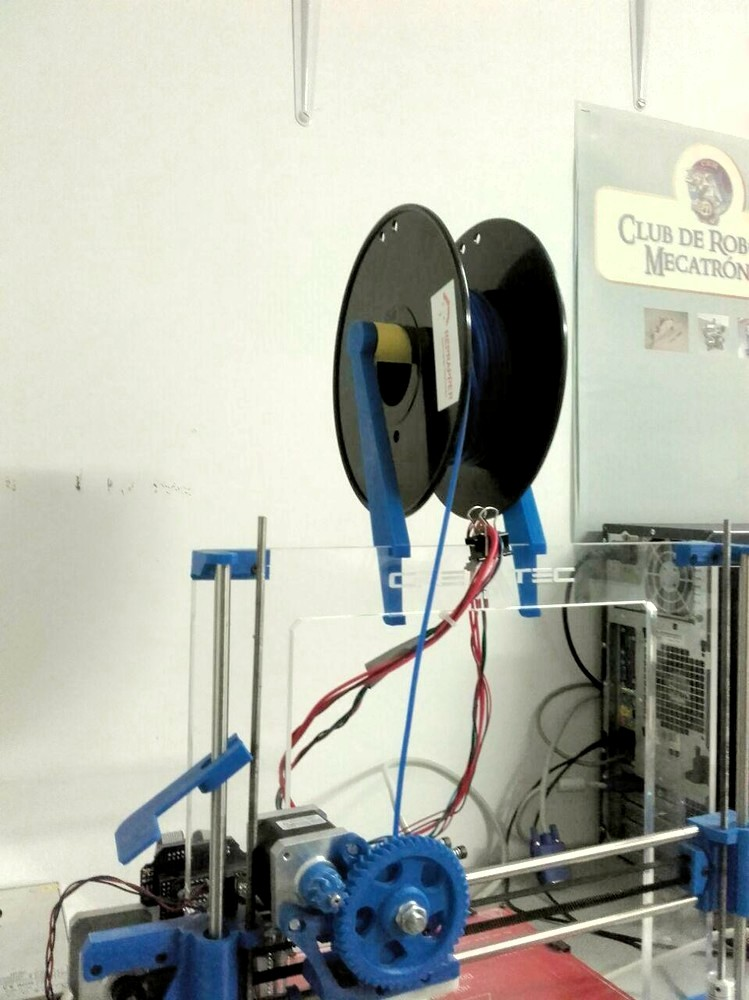
\includegraphics[width=0.3\linewidth]{fotos/filamentoImpresora}
	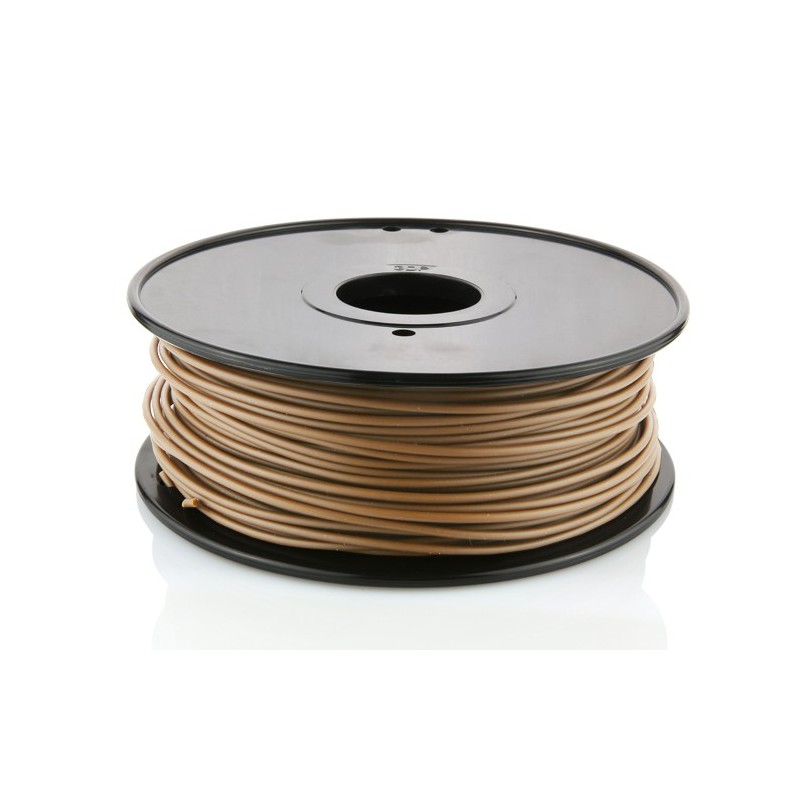
\includegraphics[width=0.4\linewidth]{fotos/filamento-madera-3mm-1kg.jpg}
	 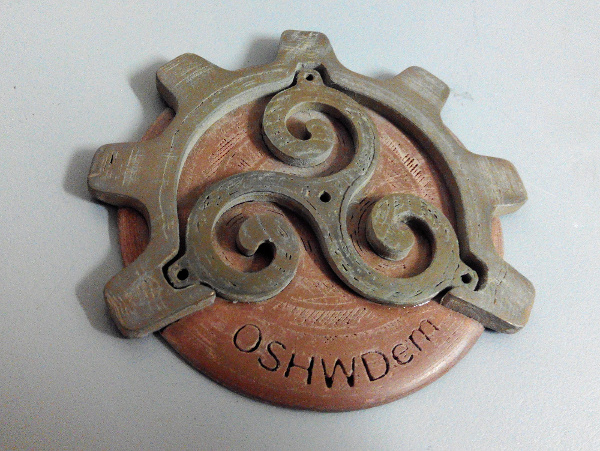
\includegraphics[width=0.4\linewidth]{fotos/trofeoOSHWDem2015.jpg}
	 }


\subsubsection{Presupuesto}

\begin{table}[htbp]
	\centering\resizebox{16cm}{!} {
		\begin{tabular}{|l|l|l|l|}
			\hline
			\multicolumn{1}{|c|}{\textbf{Producto}} & \multicolumn{1}{c|}{\textbf{Enlace de compra}}                                   & \multicolumn{1}{c|}{\textbf{Precio Unitario}} & \multicolumn{1}{c|}{\textbf{Unidades}} \\ \hline
			Bobina filamento de madera                   & \scalebox{.8}{\href{http://www.amazon.es/Ice-Filaments-ICEFIL3WOO182-Filamento-Madera/dp/B017HAIPVG/ref=sr_1_5?ie=UTF8&qid=1450094119&sr=8-5&keywords=filamento+madera+3d+3mm}{http://goo.gl/ghE447}}              & 31,90\euro{}                                        & 1                                      \\ \hline

			Bobina filameto de plástico                       & \scalebox{.8}{\href{http://www.amazon.es/gp/offer-listing/B00LXK7U40/ref=dp_olp_0?ie=UTF8&condition=all&qid=1450094934&sr=8-7}{http://goo.gl/6PKl8U}} & 19,90 + 6,90\euro{}                                        & 3                                      \\ \hline
			Laca impresora                       & \scalebox{.8}{\href{http://goo.gl/OEVBDj}{http://goo.gl/OEVBDj}} & 5,50\euro{}                                        & 1                                      \\ \hline
		\end{tabular}
	}
	\centering
	\caption{presupuesto taller de diseño e impresión 3d}
\end{table}

Lo que hace un total de \textbf{117.8\euro{}} de material fungible necesario para dar el taller de diseño e impresión 3D.

\subsection{Taller: Introducción a la robótica con Arduino}
\subsubsection{Responsables de proyecto}
\begin{itemize}
\item Carlos Garcia, alumno de doctorado, EPS.
\item Pablo Molins, personal investigador, EPS.
\item Víctor Uceda, estudiante de Informática-Matemáticas, EPS.
\end{itemize}
\subsubsection{Descripción}
Es habitual en el Club de Robótica realizar un taller prático de introducción a la robótica para los alumnos de la Escuela Politécnica Superior. Consideramos muy importante de cara al año que viene realizar este taller para dar a conocer el club a nuevos alumnos con interés en robótica pero sin conocimientos previos.
\begin{figure}[hbtp]
\centerline{
\includegraphics[width=0.33\linewidth]{fotos/2012_taller_arduino_pantallas.jpg} 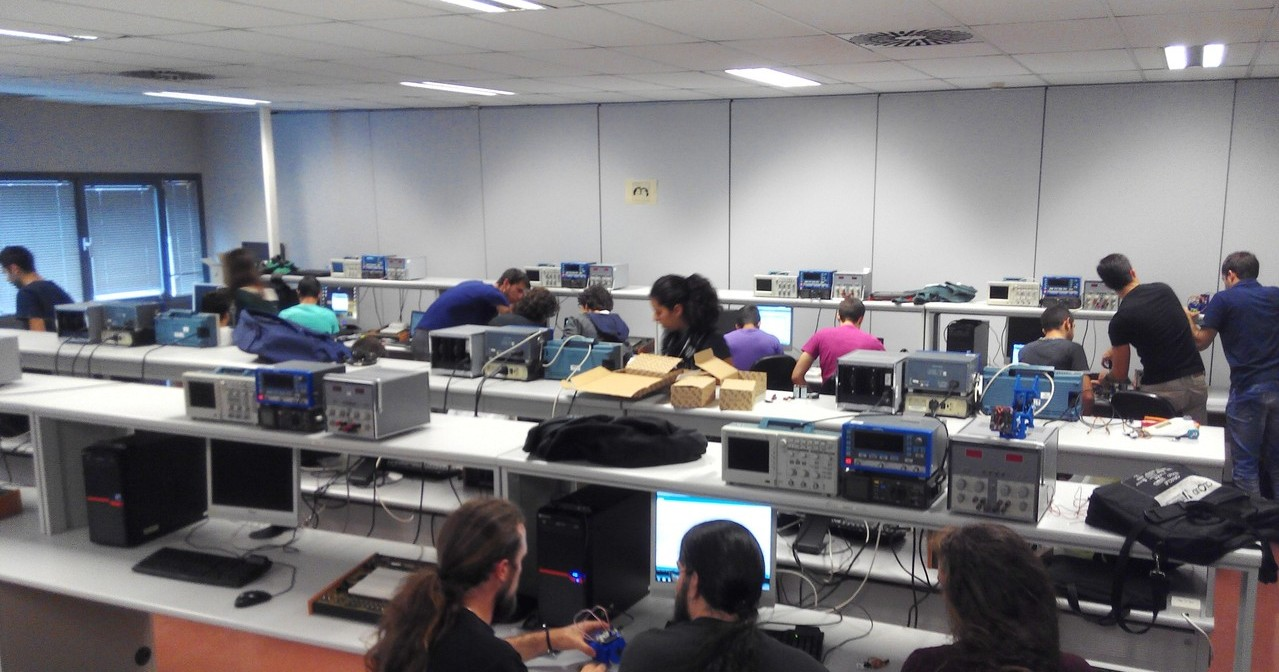
\includegraphics[width=0.4\linewidth]{fotos/fotoParticipantesArduparty.jpg} 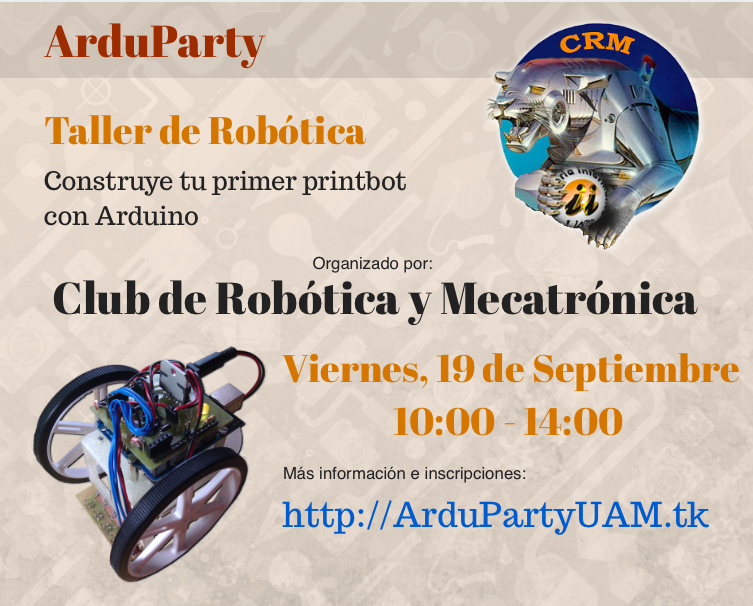
\includegraphics[width=0.33\linewidth]{fotos/2014_Cartel_ArduParty.png}}
\caption*{
Ediciones previas del taller.
}
\end{figure}

\subsubsection{Objetivos}
Seguir fomentado el conocimiento de la robótica entre los estudiantes de carreras técnicas. Dar a conocer nuestra asociación a estudiantes interesados y la nueva disponibilidad del taller del club para intentar fomentar que se creen nuevos grupos de trabajo autónomos dentro de la asociación.\\
Tenemos que seguir ofreciendo cada vez a más estudiante la posibilidad de realizar proyectos novedosos en el ámbito de la robótica y darles un pequeño empujón y respaldo necesario para llevarlos a cabo.\\
Acercar la plataforma Arduino, el diseño de Open Hardware y el diseño de estructuras 3D.
\subsubsection{Contenido}
El contenido del curso es fundamentalmente el mismo que el de la edición pasada, reutilizaremos los robots basados en la plataforma Arduino, que fueron diseñados para esa edición. Los participantes tendrán que realizar el montaje de sus kits y las conexiones eléctricas necesarias. \\
\begin{figure}[hbtp]
\centerline{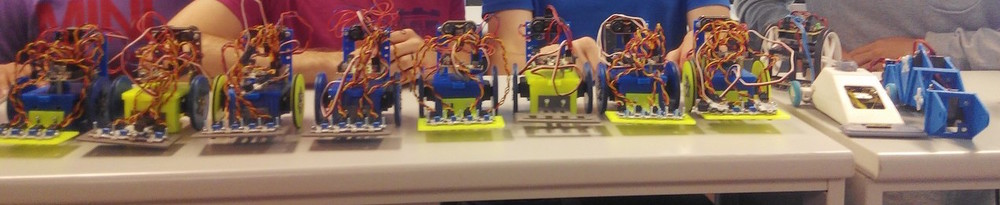
\includegraphics[width=1\linewidth]{fotos/robots_ArduParty.jpg}}
\caption*{
Robots ensamblados.
}
\end{figure}
Con el robot ya montado realizarmos diversas prácticas de programación y realizaremos interesantes retos guiando a los participantes en todo momento e introduciéndoles de esta forma en la plataforma Arduino.\\
También profundizaremos en la comunicación entre Android y Arduino (Smartphone y Robot) programando una aplicación sencilla que nos permita controlar el robot desde el móvil.

\subsubsection{Presupuesto}
Reutilizaremos los robots montados en la pasada edición del taller por lo que el presupuesto necesario es mínimo. \\
Para mejorar y suplir las deficiencias de la pasada edición necesitamos comprar baterías (pilas recargables) y cargadores para tener una mayor autonomía.\\
\begin{table}[htbp]
\centering\resizebox{16cm}{!} {
\begin{tabular}{|l|l|l|l|}
\hline
\multicolumn{1}{|c|}{\textbf{Producto}} & \multicolumn{1}{c|}{\textbf{Enlace de compra}}                                   & \multicolumn{1}{c|}{\textbf{Precio Unitario}} & \multicolumn{1}{c|}{\textbf{Unidades}} \\ \hline
Pilas Recargables 9V                    & \scalebox{.8}{\href{http://es.rs-online.com/web/p/pilas-recargables-9-voltios/7033524/}{es.rs-online.com/web/p/pilas-recargables-9-voltios/7033524/}}              & 10,28\euro{}                                        & 8                                      \\ \hline
Cargador Pilas 9V                       & \scalebox{.8}{\href{http://es.rs-online.com/web/p/cargadores-de-pilas-aaa-aa-c-d-9- voltios/5177789/}{es.rs-online.com/web/p/cargadores-de-pilas-aaa-aa-c-d-9- voltios/5177789/}} & 15,10\euro{}                                        & 2                                      \\ \hline
\end{tabular}
}
\centering
\caption{Presupuesto taller de introducción a la robótica}
\end{table}


Lo que hace un total de \textbf{112.44\euro{}} necesarios para el taller.






%\section{Organización de concursos internos y fomento de la robótica entre los estudiantes}


\section{Participación en eventos nacionales y representación de la UAM}

Hace ya años nuestra asociación, el Club de Robótica de la UAM, alcanzó grandes éxitos en competiciones de ámbito nacional como se puede ver en la recien rescatada y redactada Historia del CRM-UAM (\url{crm-uam.github.io/historia}).

Queremos, en esta nueva etapa con espiritu de refundación, volver a tener presencia en los eventos nacionales de robótica representando como se merece a nuestra universidad. Por esto presentamos los siguientes planes para participar el próximo año en los siguientes eventos.

\subsection{Liga nacional de robótica de competición. lnrc.es}
Este año (2015-16) la liga nacional de robótica de competición está inagurando la categoría de estudiantes (\url{lnrc.es/estudiantes/}). Queremos incorporarnos a esta nueva iniciativa desde el principio y presentar los robots velocistas que hemos diseñado durante los pasados cursos haciendo un rediseño específico de alguno de ellos.

Una de las ventajas de esta nueva categoria es que se brinda la oportunidad de participar con presupuestos menores que en la categoria profesional, además, no se obliga a participar en todas las pruebas de la liga pudiendo participar asistiendo a eventos puntuales.

El calendario de esta competición está publicado en la página \url{lnrc.es/comp_calendario_estu.php?an=2015-2016}.

Solicitamos presupuesto para asistir al evento {\bf Cosmobot 2016} (\url{www.roboticspot.com/cosmobot}) en Barcelona, la última prueba del calendario de la liga estudiantes.

\subsubsection{Presupuesto}
Queremos asistir como representación de la universidad en un grupo de 4 personas (por cuestión abaratamiento con habitaciones dobles y billetes con mesa en el AVE). Se presentan los siguientes precios estimados a fecha de hoy:
\begin{itemize}
\item Inscripción - Gratuita
\item Desplazamiento - AVE 55\euro{}/pers. (descuento mesa) [x4]
\item Alojamiento Hostal - 40\euro{}/noche hab. doble [x2]
\item Dietas - 20 \euro{}/pers. y día [x4]
\end{itemize}

El evento se celebra un fin de semana por lo que pretendemos asistir el sábado y el domingo, con una noche de alojamiento.

Los viajes se realizarán el sabado por la mañana la ida y el domingo por la noche la vuelta, ambos en AVE.

Solicitamos un presupuesto total para la participacion en el evento {\bf Cosmobot 2016 de 684\euro{}}

\subsection{Open Source Hardware Demostration 2016. oshwdem.org}
En el pasado noviembre se celebró la edicion 2015 del OSHWDem A Coruña. A esta pasada edición acudió de forma personal un compañero de la asociación (participando con un robot del club en un concurso de laberintos tal y como se detalla en la memoria de actividades).

Éste es un evento nacional de primer nivel, con un magnifico ambiente de colaboración entre profesionales y basado en el Open Source. Por esto creemos que la Universidad Autonóma de Madrid deberia estar representada por su asociación de Robótica en este evento en su edición del 2016.

Además es una prueba puntuable de la liga nacional de robotica de competición en la categoria de estudiantes (\url{lnrc.es/comp_calendario_estu.php?an=2015-2016}).

\subsubsection{Presupuesto}
Queremos asistir como representación de la universidad en un grupo de 4 personas (para reducir costes, ya que sirve con las plazas de un coche y alojamiento en dos habitaciones dobles). Se presentan los siguientes precios estimados a fecha de hoy:
\begin{itemize}
\item Inscripción - Gratuita
\item Desplazamiento - Coche 1200km * 0.2\euro{}/km = 240 \euro{}
\item Alojamiento - 40\euro{}/noche hab. doble [x2]
\item Dietas - 20 \euro{}/pers. y día [x4]
\end{itemize}
El evento se celebra un fin de semana por lo que pretendemos asistir desde el viernes al domingo, con dos noches de alojamiento, para poder afrontar el viaje largo en coche.

Por tanto, solicitamos un presupuesto total para la participacion en el evento {\bf OSHWDem 2016 de 640\euro{}}







\newpage



\section{Solicitud de subvención}


Como resumen de los proyectos propuestos y sus respectivos costes, a continuación proporcionamos una tabla:


\begin{tabular}{|l|l|l|}
\hline
 & \textit{\textbf{Concepto}}                          & \textit{\textbf{Presupuesto}} \\ \hline
1 & Material y herramientas para el local               & 220.15\euro{} \\ \hline
2 & Adaptación del cuadricóptero para vuelo autónomo    & 579\euro{} \\ \hline
3 & Taller: Introducción a la robótica con Arduino      & 112.44\euro{} \\ \hline
4 & Taller: Diseño e Impresión 3D (Open Hardware)       & 117.8\euro{} \\ \hline
5 & Taller: Introducción a las FPGAs libres con Verilog & 212.8\euro{} \\ \hline
6 & Construcción de un Escáner 3D modelo Ciclop         & 249.9\euro{} \\ \hline
7 & Participación en la OSHWDem A Coruña 2016            & 640\euro{} \\ \hline
8 & Participación en la LNRC Cosmobot Barcelona 2016    & 684\euro{} \\ \hline
9 & Construcción Fresadora Cyclone PCB                  & 499\euro{} \\ \hline
 & \multicolumn{1}{|r|}{\textit{\textbf{Total:}}}      & \textit{\textbf{3315.09\euro{}}}         \\ \hline
\end{tabular}


Desde la junta directiva del Club de Robótica nos comprometemos a promover todas las actividades aquí expuestas. Aún así, entendemos que el presupuesto es limitado por lo que las hemos ordenado según su prioridad, siendo primeros los conceptos más urgentes.






\end{document}
